%%**************************************************************************************************
%%
%% File Name : Main04.tex
%% 説明      : 物理学ノートの構成を明記するファイル
%%
%%**************************************************************************************************
%===================================================================================================
%  Part : 電子物性
%  説明 : 電子物性についての記述.
%===================================================================================================
    \part{電子物性}
%   %-----------------------------------------------------------------------------------------------
%   %  Input
%   %    File Name : PhysNote_SSPE.tex
%   %    説明      : 電子物性のトップファイル.
%   %              : (Solid State Physical Electronics)
%   %-----------------------------------------------------------------------------------------------
        %%**************************************************************************************************
%%
%% File Name : PhysNote_SSPE.tex
%% 説明      : 電子物性,特に半導体について学習する.
%%
%%**************************************************************************************************
%===================================================================================================
\chapter{バンド理論}
%   %-----------------------------------------------------------------------------------------------
%   %  Input
%   %    File Name : PhysNote_SSPE_Bands.tex
%   %    説明      : エネルギーバンドをシュレディンガ−方程式から導く
%   %-----------------------------------------------------------------------------------------------
        %===================================================================================================
%  Chapter : バンド理論
%  説明    : 物体の運動の表現方法について,記述する.
%===================================================================================================
%   %==========================================================================
%   %  Section
%   %==========================================================================
    \section{結晶構造}
        \begin{mycomment}
            物体は原子より構成される.原子がたくさん集まってできた塊を,私たちは
            目で見て,物体を認識しているわけだ.物体を構成している多くの原子は,
            デタラメに並んでいるわけではなく
                \footnote{
                    原子の並びを,\textbf{原子配列} という.配列とは,
                    ものが順番通りに並んでいる状態のことである.
                },
            何か一定の規則に基いている.本節では,この規則について,説明する.
        \end{mycomment}

%       %======================================================================
%       %  SubSection
%       %======================================================================
        \subsection{結晶}
            物体を構成する原子は,多くの場合,ある規則に従って並んでいる.
            この並びを,\textbf{原子配列} という.または,原子配列は \textbf{結晶構造} とも
            言われる.原子配列にはいろいろなパターンがある.以下に,その幾つかの例を挙げる.

%       %======================================================================
%       %  SubSection
%       %======================================================================
        \subsection{単位格子}

%       %======================================================================
%       %  SubSection
%       %======================================================================
        \subsection{ミラー指数}

%       %======================================================================
%       %  SubSection
%       %======================================================================
        \subsection{ブラックの回折条件}

%       %======================================================================
%       %  SubSection
%       %======================================================================
        \subsection{逆格子}

%       %======================================================================
%       %  SubSection
%       %======================================================================
        \subsection{結晶構造因子}


%   %==========================================================================
%   %  Section
%   %==========================================================================
    \section{エネルギーバンドの導出}


%       %======================================================================
%       %  SubSection
%       %======================================================================
        \subsection{トンネル効果のおさらい}

%       %======================================================================
%       %  SubSection
%       %======================================================================
        \subsection{1次元結晶}

%       %======================================================================
%       %  SubSection
%       %======================================================================
        \subsection{ペニー=クローニヒのモデル}

%       %======================================================================
%       %  SubSection
%       %======================================================================
        \subsection{ブロッホ関数}

%       %======================================================================
%       %  SubSection
%       %======================================================================
        \subsection{ブロッホの定理}

%       %======================================================================
%       %  SubSection
%       %======================================================================
        \subsection{バンドの導出}



\chapter{半導体}
%   %-----------------------------------------------------------------------------------------------
%   %  Input
%   %    File Name : PhysNote_Semiconductor.tex
%   %    説明      : エネルギーバンドをシュレディンガ−方程式から導く
%   %-----------------------------------------------------------------------------------------------
        %===================================================================================================
%  Chapter : 半導体
%  説明    : 半導体の基本的な性質を説明する.
%===================================================================================================
%   %==========================================================================
%   %  Section
%   %==========================================================================
    \section{半導体とは}
        この世界に存在する全ての物体は,電流を流すことができる.
        しかし,この電流の生じやすさは,物体ごとに異なり,電流
        が流れやすい物体と,流れにくい物体が存在する.慣習的に,
        電流の生じやすい物体を \textbf{導体} といい,電流が流れ
        にくい物体を \textbf{不導体},または \textbf{絶縁体} と
        いう.では,全ての物体が,導体か絶縁体のどちらか一方に
        分類されるかといえば,実はそうとは言い切れない.“どっち
        つかず”の性質をもつ物体もあるのだ.導体にしては電流を流し
        にくく,かといって,絶縁体というほど電流を流しにくいわけ
        でもない物体が存在するのである.このように,導体と絶縁体
        の中間のような性質をもつ物体のことを,\textbf{半導体} と
        いう.どうにも曖昧な説明だが,イメージは浮かぶだろう.
        以降では,半導体のもつ性質について考えることで,半導体を
        イメージできるよう,学習をしよう.

%   %==========================================================================
%   %  Section
%   %==========================================================================
    \section{半導体の種類}
        一口に半導体といっても,いろんな種類がある.図\ref{fig:handoutai_bunrui} に
        これを示す.
                        \begin{figure}[htbp]
                            \begin{center}
                                \includegraphicslarge{handoutai_bunrui.pdf}
                                \caption{半導体の分類}
                                \label{fig:handoutai_bunrui}
                            \end{center}
                        \end{figure}

        図からわかるように,半導体の種類を大きく分けるなら,
        2種類に分けることができる.真性半導体といわれるものと,
        外因性半導体といわれるものである.\textbf{真性半導体} とは,
        一種類の元素からなる半導体である.例えば,Si(シリコン
        ,または,珪素)や,
        Ge(ゲルマニウム)がそうである.\textbf{$i$ 型半導体} といわれ
        ることもある.
        \textbf{外因性半導体} とは
            \footnote{
                外因性半導体:\textbf{不純物半導体} ともいわれる.
            },
        複数の元素により構成される半導体である.
        有名な \textbf{$n$ 型半導体},\textbf{$p$ 型半導体} は,
        外因性半導体の一種である.

%   %==========================================================================
%   %  Section
%   %==========================================================================
    \section{キャリア(電荷担体)}
        電気伝導の発生源は,電荷の移動である.ただし,多くの場合,物質を構成する
        原子のもつ全ての電子が,電気伝導を生じさせている電荷であるというではない.
        物質を構成する原子の,周囲の電子の一部が,移動して電流が生じる.この移動
        する一部の電子のことを,\textbf{キャリア(電荷担体)} という.ところで,
        電荷には正と負の2種類あることから,キャリアにはもう一種類あることが容易に
        推察されよう.このもうひとつの正のキャリアのことを,\textbf{正孔(hole)} と
        いう.

        下に,キャリアである電子と正孔について,簡単にイメージしておこう.

%       %======================================================================
%       %  SubSection
%       %======================================================================
        \subsection{電子(electron)}
            言わずと知れた,小学生でも知っている,電子である.ただし,キャリアとし
            ての電子とは,上にも書いたように,原子を構成するすべの電子というわけで
            はない.主に,原子を構成する最外殻にある,価電子がキャリアになる場合が
            多い.

%       %======================================================================
%       %  SubSection
%       %======================================================================
        \subsection{正孔(hole)}

%       %======================================================================
%       %  SubSection
%       %======================================================================
        \subsection{電子の移動速度 と 正孔の移動速度}

%   %==========================================================================
%   %  Section
%   %==========================================================================
    \section{真性半導体の電導機構}
%       %======================================================================
%       %  SubSection
%       %======================================================================
        \subsection{Si原子の古典的イメージ}
            半導体は導体と絶縁体の中間のような性質をもつ.ここでは,半導体が導体
            として機能するときに,その電気伝導はどのように起こっているかを考える.
            それにはまず,シリコン(以降,元素記号の Si を用いて表現する)原子の構
            造を知っていることが必要である.Si原子の構造を,古典的なイメージで描
            いたのが,図\ref{fig:SiGenshi}である.
                            \begin{figure}[htbp]
                                \begin{center}
                                    \includegraphicslarge{SiGenshi.pdf}
                                    \caption{Si原子の古典的イメージ}
                                    \label{fig:SiGenshi}
                                \end{center}
                            \end{figure}
            Si原子の周囲には,14個の電子が存在している.その構成は,図のように,内
            側に2個,さらにその外側に8個,そして外周に4個である.この電子配置は,量
            子力学的に説明されるのであるが,半導体の電導機構にはあまり関係がない.
            大事なのは,一番外側に存在している4つの電子である.化学的に言えば,価電
            子と呼ばれる電子のことである.この4つの電子が結合の手になり,Si原子の共
            有結合を実現している.Siの電導機構は,この結合の手である4つの価電子の移
            動によって,説明される.以降では,最外殻電子(価電子)の個数のみが,導電
            機構に関与することから,価電子以外の電子は無視する.

%       %======================================================================
%       %  SubSection
%       %======================================================================
        \subsection{電導機構の説明}
            実際の物質は,原子ひとつではなく,複数個の原子が集まってできている.Si原子も
            同様で,多くのSi原子が共有結合している.それを模式的に表したのが,図\ref{fig:SiDendou}
            である.ただし,この図には,左右に電位を与えている.右側に正の電位を与え,左
            側に負の電位を与えている.このようにSi原子に電位を与えると,電気伝導が生じる.
            つまり,両端に電圧を加えると,電流が生じるのである.
                            \begin{figure}[htbp]
                                \begin{center}
                                    \includegraphicslarge{SiDendou.pdf}
                                    \caption{Siの電導機構イメージ}
                                    \label{fig:SiDendou}
                                \end{center}
                            \end{figure}

            この電流の電導機構は次のように説明できる.まず,電位を加えると,Si原子間の共
            有結合を担っている価電子の一部が,両側から与えられた電位によるエネルギーを受
            けとる.ネルギーを受け取った電子は,ある程度の運動量をもつようになり,Si原子
            を離れる.Si原子を離れた電子は,金属で言うところの自由電子と同じ振る舞いをす
            るようになる.この電子が,Siの電気伝導を担う電子である.ところで当然,Si原子
            から電子が離れてしまったので,そこには穴ができる.電子は負の値を持っているの
            で,開いた穴には電気的に正の性質がある.周囲の電子はこの穴を埋めるべく,移動
            してくる.そしてその穴がふさがる.そうするとまた,穴をふさいだ電子の元にいた
            場所が穴になる.さらにこの穴をふさぐべく,周囲の電子がやってくる.Siの電気伝
            導はこのように説明できる.

%       %======================================================================
%       %  SubSection
%       %======================================================================
        \subsection{常温状態のシリコンの伝導性}
            常温状態のシリコン(Si原子の塊)には伝導性がないことを計算で確認しておこう.

            シリコンのバンドギャップは1.11(\:\si{\electronvolt})である.
            一方で,室温27(\si{\degreeCelsius})から得られる熱エネルギーを計算すると,
            \begin{align*}
                kT &= 1.38  \times {10}^{-23} \times (27 + 273) (\mbox{\:\si{\joule}}) \\
                   &= 1.38  \times 300 \times {10}^{-23} (\mbox{\:\si{\joule}}) \\
                   &= 414   \times {10}^{-23} (\mbox{\:\si{\joule}}) \\
                   &= 4.14  \times {10}^{-21} (\mbox{\:\si{\joule}}) \\
                   &= 2.58  \times {10}^{-2}  (\mbox{\:\si{\electronvolt}}) \\
                   &= 0.026 (\mbox{\:\si{\electronvolt}})
            \end{align*}
            である.計算の途中で,
            \[
                1(\mbox{\:\si{\electronvolt}}) = 1.6 \times {10}^{-19}(\mbox{\:\si{\joule}})
            \]
            の換算を行った.

            よって,
            \[
                \text{リコンのバンドギャップ 1.11(\:\si{\electronvolt})} > \text{室温からの熱エネルギー 0.026 (\:\si{\electronvolt})}
            \]
            であるので,室温の熱エネルギーでは,シリコンの価電子帯の電子は伝導帯に遷移することはできない.
            つまり,シリコンは常温状態だと電流を流さない.


%   %==========================================================================
%   %  Section
%   %==========================================================================
    \section{外因性半導体の電導機構}
%       %======================================================================
%       %  SubSection
%       %======================================================================
        \subsection{外因性半導体の構成1(donor 注入)}
            外因性半導体とは,複数の元素から構成される半導体である.例えば,
            Si原子から構成される真性半導体の一部のSi原子を,価電子を5つもつ
            原子As(砒素)に置き換えると
                \footnote{
                    As(砒素)は周期表における第5族元素である.
                    第5族元素は,価電子を5つもっている.
                },
            これはn型半導体とよばれるものになる.
            このn型半導体は外因性半導体の一種である.
            図\ref{fig:SiAs}にそのイメージを示す.
                \begin{figure}[htbp]
                    \begin{center}
                        \includegraphicslarge{SiAs.pdf}
                        \caption{Si原子配列にAs(砒素)を少量埋め込む}
                        \label{fig:SiAs}
                    \end{center}
                \end{figure}

            元々,ひとつのSi原子のもつ価電子数は4つであった.そして,このSi原子
            の一部が5つの電子をもつAs原子に置き換わったのだから,単純に考えて,
                \begin{equation*}
                    (\mathrm{As}\mbox{原子の価電子数}) - (\mathrm{Si}\mbox{原子の価電子数}) = 5 -4 = 1
                \end{equation*}
            で,電子が1つ余ることになる.実は,この余った電子が外因性半導体
            の電気伝導を担う電荷なのである.

            Asの添加等により
            真性半導体中のに電子を増やすことで電気伝導性を
            高めた半導体のことを,\textbf{n型半導体} という
                \footnote{
                    nはnegative(英単語)の頭文字をとったものである.
                    英単語のnegativeには「否定的」という意味が
                    ある.電子のもつ電気量がマイナスであることから,
                    negativeが連想され,n型といわれる.
                }.

            「真性半導体にAsを注入する」ということは,「電子を注入する」
            という意味にとることができる
                \footnote{
                    実際に添加するのはAs元素なのだが,このAs添加
                    の目的は,実は,電子を注入することである.
                }.
            電子を注入するという意味で,真性半導体にAs元素を添加するとき,
            Asのこをドナー(donor)という.一般に,電子を注入するために
            添加される元素のことを \textbf{ドナー(donor)} という.

%       %======================================================================
%       %  SubSection
%       %======================================================================
        \subsection{電導機構の説明1(donor 注入)}

%       %======================================================================
%       %  SubSection
%       %======================================================================
        \subsection{外因性半導体の構成2(acceptor 注入)}

%       %======================================================================
%       %  SubSection
%       %======================================================================
        \subsection{電導機構の説明2(acceptor 注入)}

%   %==========================================================================
%   %  Section
%   %==========================================================================
    \section{ホール効果}
%       %======================================================================
%       %  SubSection
%       %======================================================================
        \subsection{ホール効果の概要}
            ホール効果(Hall effect) はHall
                \footnote{
                    Edwin Herber Hall(1855-1938, アメリカ);物理学者
                }
            が発見した電流と磁束密度に関連した現象のことである.
            1879年に発見されたといわれている.

            電流 $\bI$ が生じている導体に,この $\bI$ と直交するような
            方向に,磁束密度 $\bB$ をかける.このとき,電流 $\bI$ を担う
            キャリアは,$\bI$ と $\bB$ の両方に直交する方向にローレン
            ツ力を受ける.そうすると,導体内のキャリア密度に偏りが
            生じる
                \footnote{
                    キャリアがローレンツ力に引っ張られて,
                    導体の端のほうへ移動してしまう.
                    そうすると,導体内部にキャリアの多い部分と,
                    少ない部分が生じる.ただし,導体内キャリア
                    の,正味の個数に変化はない.
                }.
            偏ったキャリア密度は,導体の表面に電位差を発生させる.
            図\ref{fig:HallEfect1}は現象の全体像を表したものである.
            この現象を \textbf{ホール効果} という.また,ホール効果
            により生じる導体の両端の電位差を \textbf{ホール電圧} という.

                        \begin{figure}[htbp]
                            \begin{center}
                                \includegraphicslarge{HallEfect1.pdf}
                                \caption{ホール効果(イメージ)}
                                \label{fig:HallEfect1}
                            \end{center}
                        \end{figure}

%       %======================================================================
%       %  SubSection
%       %======================================================================
        \subsection{ホール効果発生の機構}
            先に,ホール効果発生のおおよその道筋を追ったが,
            ここでは,もう少し詳細に,ホール効果の発生について
            考えていこう.

            ホール効果の発生とは,ホール電圧の発生と同じことである.
            ホール電圧の発生機構を順を追って調べていこう.

            まず,発生機構を箇条書きにすれば,以下の通りになる.

                \begin{enumerate}
                    \item 導体に電流 $\bI$ が生じている
                    \item 電流 $\bI$ が生じている導体の近くに,磁束密度 $\bB$ を発生させる
                    \item 電流 $\bI$ を担うキャリアは,磁束密度 $\bB$ よりローレンツ力をうける
                    \item キャリアはローレンツ力を受け,導体内の一方向に偏る(キャリア密度に偏りが生じる)
                    \item キャリア密度の偏りにより,導体の端に電位差(ホール電圧)が生じる.
                \end{enumerate}

            また,各段階のイメージを図\ref{fig:HallEfec_Mech}に描く.

                    \begin{figure}[htbp]
                        \begin{tabular}{cc}
                            \begin{minipage}{0.5\hsize}
                                  \begin{center}
                                      \includegraphicsdouble{HallEfect2.pdf}

                                      (1)
                                  \end{center}
                            \end{minipage}
                            \begin{minipage}{0.5\hsize}
                                \begin{center}
                                    \includegraphicsdouble{HallEfect3.pdf}

                                      (2)
                                \end{center}
                            \end{minipage}
                        \end{tabular}
                    \end{figure}

                    \begin{figure}[htbp]
                        \begin{tabular}{cc}
                            \begin{minipage}{0.5\hsize}
                                  \begin{center}
                                      \includegraphicsdouble{HallEfect4.pdf}

                                      (3)
                                  \end{center}
                            \end{minipage}
                            \begin{minipage}{0.5\hsize}
                                \begin{center}
                                    \includegraphicsdouble{HallEfect5.pdf}

                                      (4)
                                \end{center}
                            \end{minipage}
                        \end{tabular}
                        \caption{ホール電圧の発生}
                        \label{fig:HallEfec_Mech} % ホール効果発生メカニズム
                    \end{figure}

%       %======================================================================
%       %  SubSection
%       %======================================================================
        \subsection{ホール効果におけるキャリアの運動}
             ホール効果における,キャリアの動きを考える.
             簡単のために,キャリア1個の運動を考える.
             ここでは,キャリアは電子(負の電荷をもつ粒子)とする.

             ホール効果は導体中に生じている電流 $\bI$ と,その
             周囲に生じている磁束密度 $\bB$ に起因する現象である.
             そこで,導体に電流 $\bI$ が生じていることと,
             その周囲に磁束密度 $\bB$ が生じていることの2点を
             仮定しよう.

%   %==========================================================================
%   %  Section
%   %==========================================================================
    \section{Schottkyダイオード}
%       %======================================================================
%       %  SubSection
%       %======================================================================
        \subsection{Schottky障壁ダイオード ダイオードの $I-V$ 特性}
        図\ref{fig:Schottky}は,通常のp-n接合とSchottky障壁ダイオードとの $I-V$ 特性の
        比較したものである.
                        \begin{figure}[htbp]
                            \begin{center}
                                \includegraphicslarge{Schottky.pdf}
                                \caption{Schottky障壁ダイオードの $I-V$ 特性}
                                \label{fig:Schottky}
                            \end{center}
                        \end{figure}

        Schottky接触ダイオードの $I-V$ 特性を考える.
        上図\ref{fig:Schottky}の $V>0$ の部分は,順バイアス
            \footnote{
                p側を正極,n側を負極に接続.
            }
        をかけたときのものである.
        このときの電流 $I$ と電圧 $V$ の関係は,
        金属から半導体へ流れる電流密度を $J_{\mbox{金属} \rightarrow \mbox{半導体}}$ として,
        \begin{align}\label{RD_1}
        J_{\mbox{金属} \rightarrow \mbox{半導体}}
        =\frac{4\pi qmk_{B}^{2}}{h^{3}}T^{2}
        \mathrm{exp}\left(-\frac{q\phi_{Bn}}{k_{B}T}\right)
        \mathrm{exp}\left(\frac{qV}{k_{B}T}\right)
        \end{align}
        が成り立つ.
        ここに,$q$ はキャリアの電気量,$\phi_{Bn}$はSchottky障壁,$m$ は有効質量,$k_{B}$ は
        ボルツマン定数,$h$ はプランク定数,$T$ は温度である.

        次に,逆バイアス
            \footnote{
                n側を正極,p側を負極に接続.
            }
        をかけたときを考える.理想的には電流は $0$ であるが,
        非常に微小な実際は電流が生じる.これは,p型半導体部分のminority carrierである
        電子がダイオードを通過するためである.図\ref{fig:Schottky}は分かりやすさのために,かなり誇張されて
        描かれている.

        図には描かれていないが,逆バイアスの電圧を徐々に大きくしていくと,
        p型半導体部分の電子が {\bf 電子なだれ} を引き起こす.この説明はタウンゼント
            \footnote{
                John Sealy Edward Townsend (1868-1957,アイルランド)
            }
        によってなされている.
        高電圧をかけるとp側の少数キャリアである電子 $e_{1}$ が大きな運動エネルギーをもち,
        半導体を構成する原子に衝突する.この衝突でその原子内部の電子 $e_{2}$ が
        飛び出す.この現象を {\bf 衝突電離} という.衝突を引き起こした $e_{1}$ は高電圧によって生ずる電場によって
        なおも運動し続ける.同様に $e_{2}$ も運動する.従って,今度は $e_{1}$ と $e_{2}$ が
        他の原子にぶつかっていって衝突電離を引き起こし,次第に大量の電子が半導体を流れていく.
        これが電子なだれと呼ばれる現象である.電子なだれが発生すると,それ以上
        大きい電圧をかけることができなくなる.

%       %======================================================================
%       %  SubSection
%       %======================================================================
        \subsection{p-n接合ダイオードのエネルギーバンド図}
        p型半導体とn型半導体を
        接触させると,
        熱平衡状態において各半導体内の電子のフェルミエネルギー
        が等しくなる.もしフェルミエネルギーが等しくならなければ
        半導体内に電流が生じるのであるが,これは外部からの
        仕事なしに電流が生じていることになり,
        すなわちエネルギー保存則に反するからである.
        従って,p-n 接合のエネルギーバンド図は
        図\ref{fig:semi_con_ketugou}のようになる.
        参考のために,接合前のn型半導体,p型半導体の
        それぞれのエネルギーバンド図を
        図\ref{fig:semi_con_bunri}に描いておく.

                    \begin{figure}[htbp]
                        \begin{tabular}{cc}
                            \begin{minipage}{0.5\hsize}
                                \begin{center}
                                    \includegraphicsdouble{semi_con_bunri.pdf}
                                    \caption{接合前}
                                    \label{fig:semi_con_bunri}
                                \end{center}
                            \end{minipage}
                            \begin{minipage}{0.5\hsize}
                                \begin{center}
                                    \includegraphicsdouble{semi_con_ketugou.pdf}
                                    \caption{平衡状態}
                                    \label{fig:semi_con_ketugou}
                                \end{center}
                            \end{minipage}
                        \end{tabular}
                    \end{figure}

        $E_{c}$ はConduction band (伝導帯) のエネルギー準位であり,
        $E_{c}$ はValence band (荷電子帯) のエネルギー隼位である.
        以降の図でもこれらの記号を用いる.


    \newpage

%       %======================================================================
%       %  SubSection
%       %======================================================================
        \subsection{Schottky障壁ダイオードのエネルギーバンド図}
        金属の仕事関数を $\phi_{m}$ とし,
        半導体の仕事関数を $\phi_{s}$ とする.
        n型半導体の場合において,
        $\phi_{m}>\phi_{s}$ のとき,金属と半導体の接触は
        Schottky接触となる.また,p型半導体の場合においてはその逆で,
        $\phi_{m}<\phi_{s}$ のときに,Schottky接触となる.

                        \begin{figure}[htbp]
                            \begin{tabular}{cc}
                                \begin{minipage}{0.5\hsize}
                                    \begin{center}
                                        \includegraphicsdouble{Shottky_p.pdf}
                                        \caption{平衡状態;p側}
                                        \label{fig:Shottky_p_bi}
                                    \end{center}
                                \end{minipage}
                                \begin{minipage}{0.5\hsize}
                                    \begin{center}
                                        \includegraphicsdouble{Shottky_p_bi.pdf}
                                        \caption{平衡状態;n側}
                                        \label{fig:Shottky_p_bi.}
                                    \end{center}
                                \end{minipage}
                            \end{tabular}
                        \end{figure}

%       %======================================================================
%       %  SubSection
%       %======================================================================
        \subsection{オーミック接触のダイオードのエネルギーバンド図}
        金属の仕事関数を $\phi_{m}$ とし,
        半導体の仕事関数を $\phi_{s}$ とする.
        n型半導体の場合において,
        $\phi_{m}>\phi_{s}$ でないとき,金属と半導体の接触は
        オーミック接触となる.また,p型半導体の場合においてはその逆で,
        $\phi_{m}<\phi_{s}$ でないときに,オーミック接触となる.

                \begin{figure}[htbp]
                    \begin{tabular}{cc}
                        \begin{minipage}{0.5\hsize}
                    \begin{center}
                        \includegraphicsdouble{ohmic.pdf}
                        \caption{平衡状態;n側}
                        \label{fig:ohmic}
                    \end{center}
                        \end{minipage}
                        \begin{minipage}{0.5\hsize}
                    \begin{center}
                        \includegraphicsdouble{ohmic2.pdf}
                        \caption{平衡状態;p側}
                        \label{fig:ohmic2}
                    \end{center}
                        \end{minipage}
                    \end{tabular}
                \end{figure}

%   %==========================================================================
%   %  Section
%   %==========================================================================
    \section{電子親和力}
    1つの原子に電子を受け入れたときに
    放出されるエネルギーのことをいう.


        \begin{table}[htbp]
            \caption{金属の電子親和力と仕事関数} \label{densin_sgotokansu}
            \begin{center}
                \begin{tabular}{|c|r|l|} \hline
                    金属 & \multicolumn{1}{c|}{電子親和力[eV]} & \multicolumn{1}{c|}{仕事関数} \\ \hline
                    Mg & 0\phantom{.}\phantom{0000} &  \\ \hline
                    Al & 0.43\phantom{00} &  \\ \hline
                    NI & 1.156\phantom{0} &  \\ \hline
                    Cu & 1.235\phantom{0} &  \\ \hline
                    Zn & 0\phantom{.}\phantom{0000} &  \\ \hline
                    Ga & 0.43\phantom{00} &  \\ \hline
                    Se & 2.0206 &  \\ \hline
                    Pd & 0.562\phantom{0} &  \\ \hline
                    Ag & 1.302\phantom{0} &  \\ \hline
                    In & 0.3\phantom{000} &  \\ \hline
                    Au & 2.3086 &  \\ \hline
                \end{tabular}
            \end{center}
        \end{table} %

    ※ 「『理科年表』,国立天文台編,丸善,2007」を参照しました.



%   %==========================================================================
%   %  Section
%   %==========================================================================
    \section{MOSFET}
%       %======================================================================
%       %  SubSection
%       %======================================================================
        \subsection{ピンチオフ効果}
        ピンチオフ効果について説明する.MOSFETは通常,図\ref{fig:MOSFET_1}に描いたような
        動作をする.この図の場合,ゲート(Gate)に正のバイアスをかけて,p型半導体に反転層
        を生成し,電子のチャネルを生成している.これにより,電子がソース側からドレイン側
        に流れることができる.
                    \begin{figure}[htbp]
                        \begin{center}
                            \includegraphicslarge{HotElectorn1.pdf}
                            \caption{通常のMOSFETの動作}
                            \label{fig:MOSFET_1}
                        \end{center}
                    \end{figure}




%===================================================================================================
%  Part : 電気回路/電子回路
%  説明 : 電気回路と電子回路の初歩を記述する.
%===================================================================================================
    \part{電気回路/電子回路}
%   %-----------------------------------------------------------------------------------------------
%   %  Input
%   %    File Name : PhysNote_EECircuit.tex
%   %    説明      : 電気回路/電子回路のトップファイル.
%   %-----------------------------------------------------------------------------------------------
        %%**************************************************************************************************
%%
%% File Name : PhysNote_EECircuit.tex
%% 説明      : 電磁気学の実際の活用例として,電気回路と電子回路について記述する
%%
%%**************************************************************************************************

%===================================================================================================
%  Chapter : 電気回路と電子回路の構成要素
%  説明    : 電気回路と電子回路をつくるのに必要な電気回路の素子;
%               ・抵抗
%               ・コンデンサ(キャパシタンス)
%               ・コイル(インダクタンス)
%               ・ダイオード
%               ・トランジスタ
%            について,記述する
%===================================================================================================
\chapter{電気回路/電子回路の構成要素}
%   %-----------------------------------------------------------------------------------------------
%   %  Input
%   %    File Name : PhysNote_EECircuit_RLCDiTr.tex
%   %    説明      : 電磁気学を構成する基本的な概念を説明する.
%   %-----------------------------------------------------------------------------------------------
        %===================================================================================================
%  Chapter : 電気回路/電子回路の構成要素
%  説明    : 電磁気学の対象となる,電気的現象・磁気的現象の実在についての確認をする
%===================================================================================================

%======================================================================
%  Section
%======================================================================
    \section{電気回路/電子回路とは何か}
    \begin{mycomment}
        「電気回路」と「電子回路」は字面だけを見る限り,一文字しか違わな
        いのだけど,両者には大きな違いがある.電気回路と電子回路を紹介
        するに当たって,最初に両者の違いを示しておくべきだろう.以下では,
        まず,電気回路にはなくてなならない要素,すなわち,導線と起電力を
        説明した後,電気回路と電子回路の違いを確認しよう.
    \end{mycomment}

    %==================================================================
    % Subsection
    %==================================================================
    \subsection{導線(導体)と絶縁体}
        この世界で,“絶対に電気を通さない物体”は存在しない
            \footnote{
                “物体は”と言うところに注意.つまり,真空でないということ.
                完全に理想的な真空は,電気を通さない.ただし,高エネルギーを
                かければ,そこから正負の電気が等量だけ発生することがあるかも
                しれないが,このノートでは,そんなあからさまに特殊な状況を
                想定することは,しない.
            }.
        電気を通す物体
        のことを \textbf{導体} と呼んでいるが,つまり,世の中のすべての
        物体は導体なのである.しかし,物体の種類は様々であり,電気の通し
        やすさは,その種類ごとに異なる.となると,当然,物体の種類の違いに
        より,電気がよく通る物体から,電気をあまり通さない物体までを順に
        並べることができる.一般的に,電気をよく通す物体を \textbf{導体} と
        いい,電気をあまり(殆ど)通さない物体のことを \textbf{絶縁体} と
        いう
            \footnote{
                絶縁体は,不導体(ふどうたい)とも言われる.
            }.
        そして,\textbf{導線} とは,導体を細長い紐状に整形したもののこと
        をいう.

        “よく通す”だとか,“あまり通さない”とかと書いてしまったが,
        この「よく」と「あまり」とは,具体的にどういうことかは,説明
        していない.つまり,導体と絶縁体の区別が曖昧に扱ってしまっている.
        そこで,差し当たっての理解として,乾電池と豆電球を何か物
        体でつないだ時,豆電球が光るなら,その物体は導体である,と判
        断して貰って構わない.というか,このノートでは,その程度の理
        解で十分だし,実際に電気回路を作って遊ぶ場合にも,これ以上の
        知識は必要としない.

        実は,導体と絶縁体を明確に区別するような定義は存在しない.
        そもそも,電気の流しやすさというものは,世の中に存在する
        物体の種類すべてに対して,相対的にしか評価できない.
        しかし,多くの場合,\textbf{電気抵抗率} という概念を持ち出して
            \footnote{
                電気抵抗率については,\ref{subsub:teikou_ritu}節を参照.
            },
        その値により,おおよその区別がなされる.例を以下に示しておこう.
        実際の具体的な数値は物質ごとに様々であるので,そのオーダー(桁数)
        による区別する.

        \begin{center}
            \begin{tabular}{lllll}
                導体    &:  & ${10}^{-8}$ & [$\Omega$m] & 以下 \\
                絶縁体  &:  & ${10}^{8}$  & [$\Omega$m] & 以上
            \end{tabular}
        \end{center}
        \begin{figure}[hbt]
            \begin{center}
                \includegraphicslarge{DouTaiZetsuenTai_Kubetu.pdf}
                \caption{導体と絶縁体の抵抗率}
                \label{fig:DouTaiZetsuenTai_Kubetu}
            \end{center}
        \end{figure}

        このように書いてしまうと,導体と絶縁体の間の電気抵抗率の値を持つ物体は
        ないのか,といった質問がしたくなるだろう.とりあえず,これに回答しておこう.
        そのような物体は存在し,実際に \textbf{半導体} と言われていて,現在の
        コンピュータを構成するためにもっとも重要な役割を担っている.図に加えておこう
        (図\ref{fig:DouTaiHandouTaiZetsuenTai_Kubetu}).
        \begin{figure}[hbt]
            \begin{center}
                \includegraphicslarge{DouTaiHandouTaiZetsuenTai_Kubetu.pdf}
                \caption{導体と半導体と絶縁体の抵抗率}
                \label{fig:DouTaiHandouTaiZetsuenTai_Kubetu}
            \end{center}
        \end{figure}

        導体には自由電子と呼ばれる,原子核に束縛されていない電子が多数存在
        している.この自由電子こそが,電気を通す役割をになっている.自由電
        子は導体中に多数存在するが,それら全体の動きが,電流として認識され
        る.これに対し,絶縁体には自由電子は存在しない.これが,導体と絶縁
        体の性質が大きく異なる,直接の原因である.しかし,何度も言うが,
        絶縁体であっても電流は,微弱とみなされてしまうが,生じる.これは絶
        縁体の抵抗率が有限であることからも,根拠付けられる
            \footnote{
                電流を生じさせない,完全な絶縁体であれば,電気抵抗率は無限
                大であり,測定不可能でなければならない.しかし,現実には,
                電気抵抗率が無限大となるような物質の存在は確認されていない.
            }.

        \begin{memo}{導体/半導体/絶縁体の違い}
           導体と半導体,絶縁体の違いは,どこから生じてくるのだろうか
               \footnote{
                   「自由電子の存在の有無」がその根拠であるが,もう少し,
                   立ち入って考えてみよう.
               }.
           電気抵抗率は物質の種類による物理定数のひとつだが,
           その値のとりうる範囲は,あまりにも広すぎる.物理
           学における他の物理定数の中でも,屈指の範囲の広さ
           である.この物質によって大きく値の異なる電気抵抗
           率は,古典的に説明しようとしても,成功することは
           ない.つまり,量子論を使わないと,説明のつかない
           現象なのである.言い方を変えれば,この電気抵抗率
           の値は,量子論を使うことによって説明のつく現象で
           ある.それは,エネルギーバンドという概念を用いる
           ことで,直感的に説明がなされる.エネルギーバンド
           を可視化した図が,
           図\ref{fig:Energy_Band_DHZ}である.
           \textbf{エネルギーバンド図} ,または,誤解が生じるおそれがない場合には,
           単に \textbf{バンド図} ということが多い.
               \begin{figure}[hbt]
                   \begin{center}
                       \includegraphicslarge{Energy_Band_DHZ.pdf}
                       \caption{導体と半導体と絶縁体のバンド図}
                       \label{fig:Energy_Band_DHZ}
                   \end{center}
               \end{figure}

           図\ref{fig:Energy_Band_DHZ}の左側が絶縁体のバンド図である.
           禁制帯の幅
               \footnote{
                   禁制帯の幅:価電子帯と伝統帯との最小のエネルギー差
                   のこと.単位の[eV]はエレクトロンボルトとよむ.
                   1[eV]は,1[V]の電位差がある空間内で電子1つがもっている
                   エネルギーである.
               }
           が,6[eV]以上あれば,絶縁体とみなしてよいだろう.
           図\ref{fig:Energy_Band_DHZ}の真ん中が,半導体のバンド図
           である.禁制帯の幅が,1$\sim$[eV]前後であれば,半導体と
           いってよいだろう.導体のバンド図は,図\ref{fig:Energy_Band_DHZ}の
           右側である.注目するのは,伝導帯と半満帯ここには,自由電子が
           多数存在するエネルギー帯である.

           導体と半導体,絶縁体の区別を理解した段階で,
           エネルギーバンド図はどのように得るのか,という疑問が生じると思うが,
           これについては,物性の部分で考えることにしよう.電気回路や電子回路
           を学ぶには,あまり関係がないのである.このエネルギーバンドの説明だ
           って,あまり関係がないのに---.
        \end{memo}


    %==================================================================
    % Subsection
    %==================================================================
    \subsection{起電力$\cdot$電源}
    \subsubsection{起電力}
        導線の両端に電位差を生じさせるもののことを,\textbf{起電力} という.
        導線の両端に電位差が生じれば,その導線内部の自由電子は運動を始めて,
        電流が生じる.回路に電流を生じさせるためには,起電力が必要なのである.

        もう少し詳しく説明しよう.
        導体からなる導線には,多数の自由電子が存在している.
        しかし,導体のみが存在していても,その導体中に電流が生じることはない
            \footnote{
                導体内の自由電子の配置が一意的に定まることと,
                エネルギー保存の法則からの帰結である.
            }.
        なので,電気回路に電流を生じさせるには,導線にエネルギーを与えてる
        必要がある.つまり,導線の両端に電位差を生じさせないといけないのだ.

        電流とは,導線内の多数の自由電子の平均的な移動とみなせるから,
        導線に電流が生じるためには,その内部の自由電子に速度を与えれば
        よい.導体内の自由電子が速度を持つようなエネルギーの与え方なら
        ば,その与え方はどのようであっても構わない.例えば,トムソン効果
            \footnote{
                トムソン効果:導線の両端の一方に高熱源を接触させ,他方に
                低熱源を接触させる.すると,導線の両端に温度差が生じる.
                このとき,温度の高い方から低い方に向かう向きに起電力が生じ
                (これを \textbf{トムソン効果} という),電流が生じる.
                熱力学の第二法則によれば,
                このように熱の分布に偏りが生じる場合,それを熱平衡状態に
                なるように,熱分布の変化が起こる.
                導線のもつ熱の原因の1つに,自由電子の運動エネルギーが挙げられる
                (当然ながら,導線を構成する導体の原子核の振動も,
                その原因のひとつに挙げられるが,電流が生じる原因としては
                関係がないので,ここでは無視する).
                つまり,温度の高い方の自由電子のが,温度の低い方へ移動
                するのである.これが,電流として観測されるのである.

                \ref{subsec:ThomsonEffect}節(\pageref{subsec:ThomsonEffect}ページ)参照.
            }
        を狙って,導線の両端に温度差を作ったりしてもいいし,電磁誘導を狙って,
        導線を一様な磁場中を運動させてもいい.しかし,一番手っ取り早く,簡単に
        イメージできるのは,乾電池につなぐことである.とにかく,導線の両端に
        電位差を生じさせ,導体内部の自由電子にエネルギーを与えるのである.
        起電力とは,エネルギーの源であり,回路はこの起電力から得たエネルギーを
        自由電子の運動エネルギーとして受け取るのである.

    \subsubsection{電源}
        起電力が電気回路,あるいは,電子回路を作動させるためのエネルギー源
        として使用されるとき,この起電力は別名として,\textbf{電源} という
        のが一般的である.

    \begin{memo}{起電力と電源の違い}
        起電力を得るには,乾電池を使用するのが一番簡単な方法だ.
        手動のダイナモ発電機を使用するのも面白い(自転車のライト等).
        乾電池や発電機は具体的に目に見える物として存在する.だから,
        電気回路図として乾電池や発電機を記号化して,その位置を描くこと
        ができる.

        しかし,起電力を得るには,電磁誘導を直接的に利用する方法も
        考えられる(図\ref{fig:kidenryoku_Dengen01}参照).
            \begin{figure}[hbt]
                \begin{center}
                    \includegraphicsdefault{kidenryoku_Dengen01.pdf}
                    \caption{電磁誘導による起電力}
                    \label{fig:kidenryoku_Dengen01}
                \end{center}
            \end{figure}

        図\ref{fig:kidenryoku_Dengen01}の右側の回路に,電磁誘導により
        起電力が生じて電流が流れ始めるのだが,具体的にどこに起電力が存在
        するかを示すことは不可能である.つまり,起電力の発生場所の特定が
        できないので,電気回路図に描き難いのである
            \footnote{
                電磁誘導の法則によれば,起電力はコイル全体に生じている
                のだが,コイルそれ自体は電源でも起電力でもない.
                あくまでも,外部の磁場の時間変化に反応するだけ意である.
            }
        いうなれば,回路全体
        に起電力が生じたと言うのが,最も適切な表現だろう.
        「起電力」とは,「電源」をその一部として含む,より範囲の広い言葉
        として考えたほうが良いかもしれない.電気回路で使用される起電力の
        ことを『電源』という,認識よいと思う.
    \end{memo}

    %==================================================================
    % Subsection
    %==================================================================
    \subsection{電気回路}
        電気回路とは何かを,一般的に言葉で説明するのは難しいし,例えそれが
        できたとしても,何か難しい言い回しになってしまいかねない.そこで,
        ここでは具体例を挙げることで,電気回路についてのイメージを捉えること
        としよう.

        小学生の頃,豆電球と乾電池を用意して,それらをつなぎあわせて,
        豆電球を光らせた経験があるだろう.これが,最も単純な電気回路
        と言える.

        もっと複雑な電気回路も経験しているだろう.コイルを作成して,
        モータ,もしくは電磁石,ダイナモ発電機などを作ったことはな
        いだろうか.これらを使った回路も,電気回路である.

        コイルや豆電球などを使って,それらを起電力につなぎ,
        電流が一周できる状態になったものが電気回路である,
        と言える.

        \begin{memo}{理論が先か.経験が先か}
            電気回路とは何か.この疑問を解決させるには,世の中で電気回路
            と言われるものに触って,実感するのが手っ取り早い.理論的なこと
            は,そのあとで学べば良い.しかし,現実問題として,紙と鉛筆だけ
            を使って,電気回路の教科書をよむ場合には,予め電気回路というも
            ののイメージを持っていないと,理解するのに大変に時間がかかるだ
            ろう.理論とは,あくまでも,現実に起きている現象を説明するためのも
            のであり,私たちの経験をもとに構築される.つまり,理論を学ぶ前に,
            実際に体で経験していることが,最も望ましい学習スタイルである.
            (にもかかわらず,大学などの学生実験では,実験に先立って,理論の
            学習を迫られる.何かおかしい気がしてならない.“時間の都合”と
            して,片付けられてしまうのだろうか.)
        \end{memo}

    %==================================================================
    % Subsection
    %==================================================================
    \subsection{電子回路}
        電子回路を一言で言い表すことは,電気回路と同じで,とても難しい.
        ましてや,電子回路は電気回路と違って,小学生の頃から馴染みのある
        というものではなく,ともすると,見たことも聞いたこともない人も
        いることだろう.なので,初めて「電子回路」という単語を聞いたとい
        う方は,この節を読み飛ばして,先に進んでもらいたい.そうすれば,
        電子回路についてのイメージが,徐々に湧いてくることだろう.

        電子回路の例として,例えば,交流を直流に変えるインバータや,
        またはその逆作用であるコンバータ(直流を交流に変える)がある.
        また,オペアンプを使った各種演算回路も,電子回路と呼ばれる
        ものである.

        要するに,回路内の電流や電圧をその回路自身で制御して,自らの
        動き方に変化を加えれるような回路のことを,電子回路という.
        インバータの例で言えば,起電力の向きが負の向きになったと
        判断して,その方向を逆転させて正方向になるように,自身の
        動きを制御させることができる,ということである.
        こういう意味から,電子回路は能動的な回路と言われることもある
            \footnote{
                電子回路が能動的な回路と呼ばれるのに対し,
                電気回路は受動的な回路と言われる.電気回路は
                一定の動きしかできない.変化を見たい場合には,
                起電力の与え方を変える(起電力の出力波形
                を変化させるということ)必要がある.起電力
                に対して受動的という意味で,このように呼ばれるのだ.
            }.

        よりはっきりとした電子回路のイメージを得るには,実際に作って
        みるか,学習を進めていくかしかない.具体的な電子回路を多くみる
        ことで,電子回路のイメージが身につくことだろう.

    %==================================================================
    % Subsection
    %==================================================================
    \subsection{電気回路と電子回路の違い}
        先にも書いたが,電気回路と電子回路には大きな違いがある.
        電気回路は起電力に対して,一定の動作をさせることしかできないが,
        電子回路はそれ自身の動きに変化を加えることができる.例えば,
        一定方向の電流しか通さない(ダイオード)であるとか,振動する入力
        信号に対して,ある周波数領域の信号しか通過させない(ほかは遮断する)
        とかといったもが電子回路である.

        電気回路は起電力に対して受動的であり,電子回路は能動的に反応する.
        具体的なイメージが湧かず,モヤモヤした気分かもしれないが,ここで
        止まってしまっては,先に進めない.学習を先に進むことで,分かってくるこ
        とであり,具体例をたくさん見ることが,理解を早めるために
        必要である
            \footnote{
                当然ながら,闇雲に先に進んでも得るものはない.
                適切な参考書,雑誌,教科書,友人,指導者などを頼りに,
                学習を進めないとならない.
            }.
        多少のモヤモヤ感を押さえ,先に進もう.

%======================================================================
%  Section
%======================================================================
    \section{電気回路の構成要素}
    %==================================================================
    % Subsection
    %==================================================================
    \subsection{素子}
        電気回路や電子回路を構成する基本的な構成要素は,以下に書くように
        いくつかあるが,それらを総称して,\textbf{素子}(そし)という
            \footnote{
                素子:「そし」と読む.「もとこ」ではありません.
            }.
        電気回路を構成するのに必要な素子は3種類ある
            \footnote{
                たった3つしかない,といったほうがいい(驚きを込めて).
                3種類の素子だけで,バリエーションにとんだ,様々な動作を
                する電気回路を作ることができる.
            }.
        それらは,
            \begin{enumerate}
                \item 抵抗
                \item キャパシタ(コンデンサともいわれる)
                \item インダクタ(コイルともいわれる)
            \end{enumerate}
        と呼ばれている.

        次節から,この3つの素子(抵抗,キャパシタ,インダクタ)
        とは何かといった説明と,数学的解析を行うための定義を紹介する.

        ちなみに,電子回路を構成する素子は5種類である.上の電気回路の3
        種類に加えて,ダイオードとトランジスタが使われる.
        また後に,改めて,紹介しよう.

    %==================================================================
    % Subsection
    %==================================================================
    \subsection{抵抗とオームの法則}
    \subsubsection{抵抗の定義}
        まず,最も単純で基本的な素子である \textbf{抵抗} について考える.
        小学生の頃から,あるいは中学生の頃からおなじみの,
        \textbf{オームの法則} を確認する.
        この法則は以下のようである.
            \begin{myshadebox}{オームの法則}
                導体に流れる電流 $I$ と,そのときの導体にかかる
                電圧 $V$ は比例関係にある.
                式で表現すれば,その比例定数を $R$ として,
                    \begin{align}
                        V=RI
                    \end{align}
                である.この比例定数は導体の状態や種類によって異なる.しかし,
                同一の導体で状態も同じであれば,抵抗値は一通りに決まる.
            \end{myshadebox}

        この比例定数 $R$ を \textbf{抵抗} (Resistance)という.
        この法則から,電流と抵抗から電圧が計算できる.また,電圧と抵抗から電流が計算できる.
        論理的に整理しようとすると,電流を電圧と抵抗によって定めるか,もしくは,電圧を電流と
        抵抗で定めるかを決めないといけない.しかし,どちらをとっても,論理的整合性はよくない.
        そこでここでは,この法則は,「電流と電圧の比例関係を表現する法則」であるという解釈に
        とどめておく.

    \subsubsection{抵抗の回路図記号}\label{subsub:kairozu_kigou_teikou}
        電気回路を,紙面上に書く場合,抵抗は次のように表現される.
                    \begin{figure}[hbt]
                        \begin{center}
                            \includegraphicsdefault{kairozu_kigou_teikou.pdf}
                            \caption{抵抗の回路図記号}
                            \label{fig:kairozu_kigou_teikou}
                        \end{center}
                    \end{figure}

        図\ref{fig:kairozu_kigou_teikou}は最も基本的な,抵抗を
        表す記号である.実際の抵抗には,抵抗値を変更できる可変抵抗器や,
        高電力用のホーロー抵抗器などがあり,それらには別の記号が割当て
        られている.

    %==================================================================
    % Subsection
    %==================================================================
    \subsection{キャパシタ}
    \subsubsection{キャパシタの物理的構成}
        物理学では,コンデンサとは,二つの物体が互いに近くに存在するとき,
        この一対のことをいう.
                    \begin{figure}[hbt]
                        \begin{center}
                            \includegraphicsdefault{condenser.pdf}
                            \caption{コンデンサ}
                            \label{fig:condenser}
                        \end{center}
                    \end{figure}

        このコンデンサは,電気回路においては,理想的な素子
        という意味で,\textbf{キャパシタ} とよばれることが多い.
                    \begin{figure}[hbt]
                        \begin{center}
                            \includegraphicsdefault{capacita_idea.pdf}
                            \caption{キャパシタンスの最も簡単なイメージ}
                            \label{fig:capacita_idea}
                        \end{center}
                    \end{figure}

    \subsubsection{キャパシタンスの定義}
        キャパシタンスとは,簡単にいえば蓄電器
            \footnote{
                蓄電器:電気をためておくことのできる装置のこと.
            }
        である.もう少し細かくいうと,キャパシタンスとは
        ある電圧 $V$ に対して溜まる電気量 $Q$ のことをいう.
        式で書けば以下の通りである.
            \begin{myshadebox}{キャパシタンスの定義}
                キャパシタンス $C$ は,その両端に電位差 $V$ を与えたときに,
                それに蓄えられる電気量 $Q$ のたまり具合で定義される.
                \begin{align}
                    C:=\frac{Q}{V}.
                \end{align}
            \end{myshadebox}

    \subsubsection{キャパシタの回路図記号}\label{subsub:kairozu_capacita}
        キャパシタンスの電気回路記号は,
        図\ref{fig:kairozu_capacita}の通りである.
                    \begin{figure}[hbt]
                        \begin{center}
                            \includegraphicsdefault{kairozu_capacita.pdf}
                            \caption{キャパシタンスの回路図}
                            \label{fig:kairozu_capacita}
                        \end{center}
                    \end{figure}

    \subsubsection{キャパシタの電気回路中の動作}
        キャパシタは電気回路の素子であるから,
        電流と電圧に対してどのように作用するかを考えておく必要がある.
        電流を $I$ と表現することにしよう.
        電磁気学では電流の向きをベクトルで表現していたが,
        電気回路の部分では,電気回路の方向に電流が生じることはわかりきっているので,
        その大きさのみを扱うことにする.
        電流とは電荷の動きそのものであった.
        つまり,電流  $I$ は電荷の時間変化で表現できて,
            \begin{align}
                I=\frac{\df Q}{\df t}
            \end{align}
        である.両辺を時間 $t$ で積分すると,
            \begin{align}
                \int I\,\df t&=\int \left(\frac{\df Q}{\df t}\right) \,\df t
                =\int \df Q  \\ \notag \\ \notag
                \therefore\quad Q&=\int I\,\df t
            \end{align}
        である.これを,キャパシタンスの定義式に代入すれば,
            \begin{align}
                C=\frac{1}{V}\int I\,\df t
            \end{align}
        となる.

        このノートでは,オームの法則を電圧 $V$ について解いた式で表現したので,
        キャパシタンスについても同様に統一すれば,
            \begin{align}
                V=\frac{1}{C}\int I\,\df t
            \end{align}
        である.

        また,電流について解くと,
            \begin{align}
                \int I\, \df t &= CV \notag \\
                \quad \therefore \quad
                I &= C \frac{\df V}{\df t}.
            \end{align}

        まとめておこう.
            \begin{myshadebox}{キャパシタンスと電流$\cdot$電圧の関係}
                キャパシタンス $C$ と,電流 $I_{C}$,電圧 $V_{C}$ の関係
                    \footnote{
                        電流と電圧の添字につけた $C$ は,それぞれ,
                        キャパシタを流れる電流とキャパシタの両端の
                        電位差を強調するために,付加した.
                    }
                は,以下のようになる.
                \begin{align}
                    V_{C} = \frac{1}{C}\int I_{C}\,\df t
                    \,,\quad \mbox{または},\quad
                    I_{C} = C \frac{\df V_{C}}{\df t}.
                \end{align}
                上の二つの式は,回路方程式をたてる際に使用する.
                この式は,キャパシタンスに対する,オームの法則に
                相当するものと考えてもいい.
            \end{myshadebox}

    %==================================================================
    % Subsection
    %==================================================================
    \subsection{インダクタ}
    \subsubsection{インダクタの物理的構成}
        知ってのとおり,コイルとは導線を円筒状に巻いたものである.
                    \begin{figure}[hbt]
                        \begin{center}
                            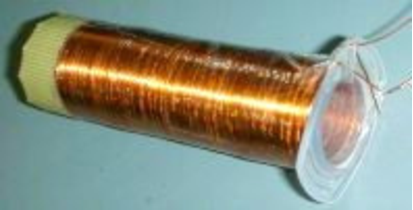
\includegraphics[keepaspectratio, width=50mm,height=25.6mm,clip]{koiru1.pdf}
                            \caption{インダクタ(コイル)}
                            \label{fig:koiru1}
                        \end{center}
                    \end{figure}

        コイルを電気回路に用いるとき,理想的なコイルというよな意味で,
        \textbf{インダクタ} という用語を用いる
            \footnote{
                インダクタにも種類があって,
                主なものには無限に長い円筒状のものを \textbf{ソレノイド},円環状(ドーナツ状)にした
                ものを \textbf{トロイダル} という.
            }.

    \subsubsection{自己インダクタンスの定義の準備}
        インダクタにおける電流と電圧の関係を考える.
        インダクタの原理の根底には,ファラデーの電磁誘導の法則がある.
        この法則は,電磁気学で学習したように,
            \begin{align}
                V=-\frac{\rd \Phi }{\rd t}
            \end{align}
        である.ここに,$\Phi (t)$ は磁束である.電磁気学では
        電場と磁束密度で電磁誘導の法則を表現したが,
        電気回路では電圧(起電力)と電流の関係を調べたいので,
        上のような表現を用いる.

        ソレノイド状のコイルが作る磁束は電流を用いて $\Phi=NS\mu_{0}I/l$ である.
        ここに,$N$ はコイルの巻数,$S$ はコイルの断面積,$l$ はコイルの長さである.
        従って,これを電磁誘導の法則 $V=-\df \Phi/\df t$ に代入すると,
            \begin{align}
                V=-\frac{\df \Phi}{\df t}=-\frac{\df }{\df t}\left( \frac{NS\mu_{0}}{l}I \right) =-\frac{NS\mu_{0}}{l} \frac{\df I}{\df t}
            \end{align}
        となる.ここで定数の部分を,ソレノイドコイルの \textbf{自己インダクタンス} $L$ と定義する.
        すると,コイルの両端の部分の電位差は
            \begin{align}\label{eq:L_Define}
                V=-L\frac{\df I}{\df t}
            \end{align}
        となる.

        または,電流について解くと,
            \begin{align}
                I=-\frac{1}{L} \int V\,\df t.
            \end{align}

    \subsubsection{自己インダクタンスの定義}
        自己インダクタンスについての解説は,上記の通りである.
        しかし,ここで,自己インダクタンスの符号を逆転しておきたい.というのも,
        電磁気学的に学んだ場合(上記の場合)には,
        自己インダクタンスの符号を負として扱う.これは,
        自己インダクタンス自身を基準にした見方であり,外からの磁束の変化に逆らうとして
        (レンツの法則)いるからである.つまり,コイルが外部に対してどのように作用するかに
        視点が置かれていたのである.しかし,\textbf{電気回路理論においては,外からの電圧が
        基準になる}.なので,自己インダクタンスの定義が異なり,符号が逆転することになる.
        要するに,
            \begin{align*}
                L_{\mathrm{EM}} = -L_{\mathrm{ECirc}}
            \end{align*}
        である.ここに,$L_{\mathrm{EM}}$ は電磁気学的(Electro Magnetism)な自己インダクタンスを表し,
        $L_{\mathrm{ECirc}}$ は電気回路論的(Electric Circuit)な自己インダクタンスを表している.
        すると,関係式の符号も逆転し,以下のようになる.
            \begin{align}
                V=L\frac{\df I}{\df t}
                \,,\quad
                I=\frac{1}{L} \int V\,\df t.
            \end{align}
        一般的に
            \footnote{
                論理がかなり飛躍する.
            },
        電圧が電流の時間変化に比例する場合
            \footnote{
                要するに,式(\ref{eq:L_Define})が成り立つとき.
            },
        その比例定数を \textbf{自己インダクタンス} とよぶ.
            \begin{myshadebox}{自己インダクタンスの定義}
                電圧 $V_{L}$ が電流 $I_{L}$ の
                    \footnote{
                        電圧と電流の添字 $L$ は,それぞれ,自己インダクタンスの
                        両端の電圧とインダクタに生じる電流を強調するための
                        ものである.
                    },
                時間変化に比例する場合
                    \footnote{
                        強磁性体(Fe,Co,Ni)などは,磁束密度中に置かれると
                        磁化してしまう.この場合,比例関係は成立しない.
                        つまり,インダクタの構成物質に強磁性体を含んでいるならば,
                        自己インダクタンスを定義することは難しい.
                    }
                その比例定数 \textbf{自己インダクタンス} といい,
                これを $L$ と記述する.この時に成り立つ式は,以下の通り
                である.
                \begin{align}
                    V_{L}=L\frac{\df I_{L}}{\df t}
                    \,,\quad \mbox{または},\quad
                    I_{L}=\frac{1}{L} \int V_{L} \,\df t.
                \end{align}
                インダクタに流れる電流が,自身の両端の電位差に影響を
                及ぼしている.インダクタ特有の現象を,\textbf{自己誘導} と
                いう.
            \end{myshadebox}

        \begin{memo}{ソレノイドのつくる磁束密度}
        ソレノイド上の導線が作る磁束密度を,物理法則を用いて,
        導出してみよう.
                \begin{figure}[hbt]
                    \begin{tabular}{cc}
                        \begin{minipage}{0.5\hsize}
                        \begin{center}
                            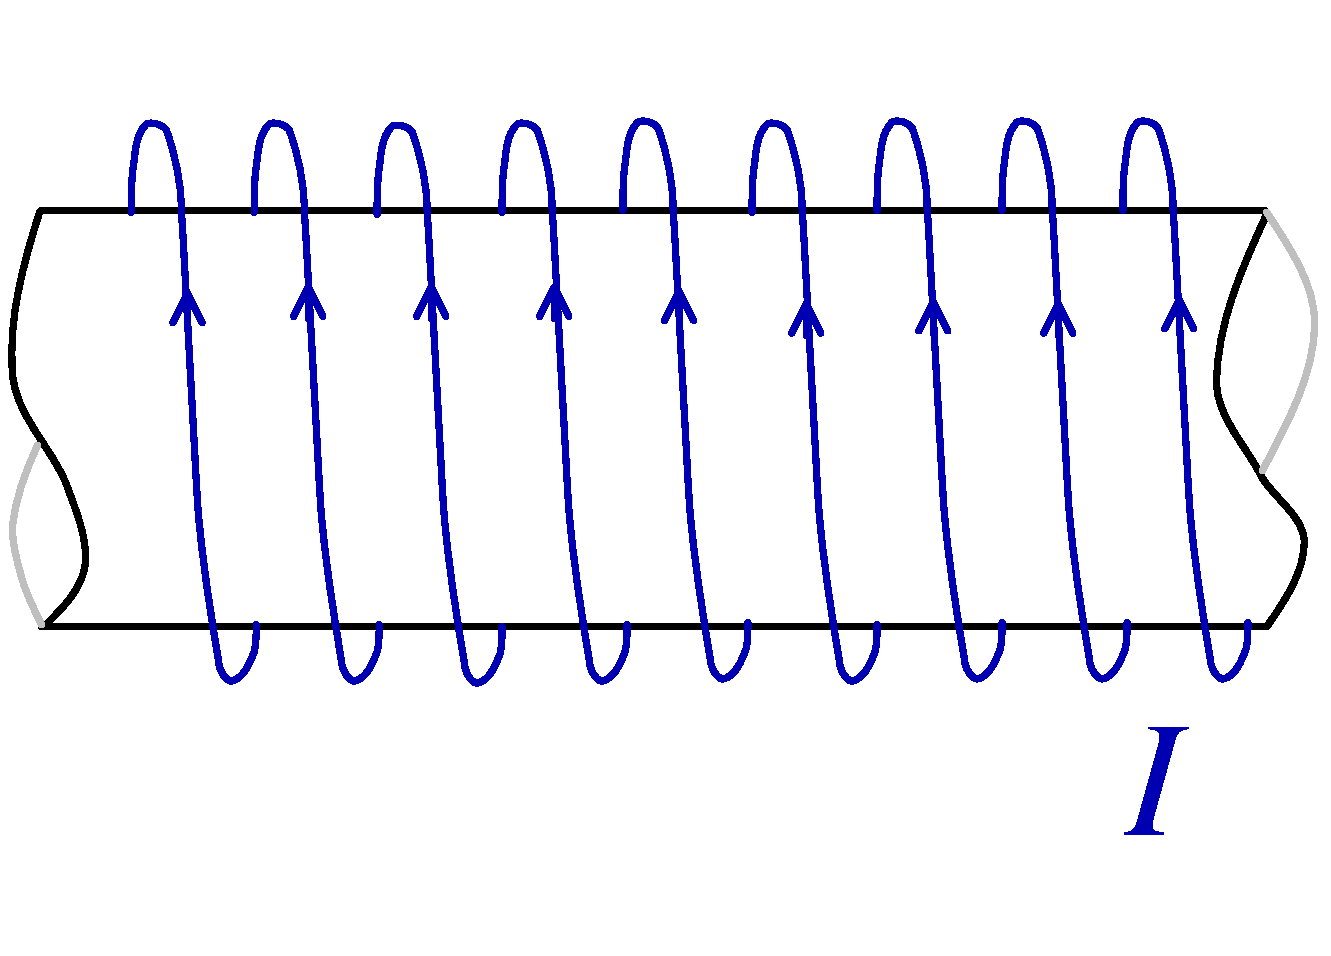
\includegraphics[keepaspectratio, width=3.5cm,height=2.8cm,clip]{sorenoido11.pdf}
                            \caption{ソレノイド(外観)}
                            \label{fig:sorenoido11}
                        \end{center}
                        \end{minipage}
                        \begin{minipage}{0.5\hsize}
                        \begin{center}
                            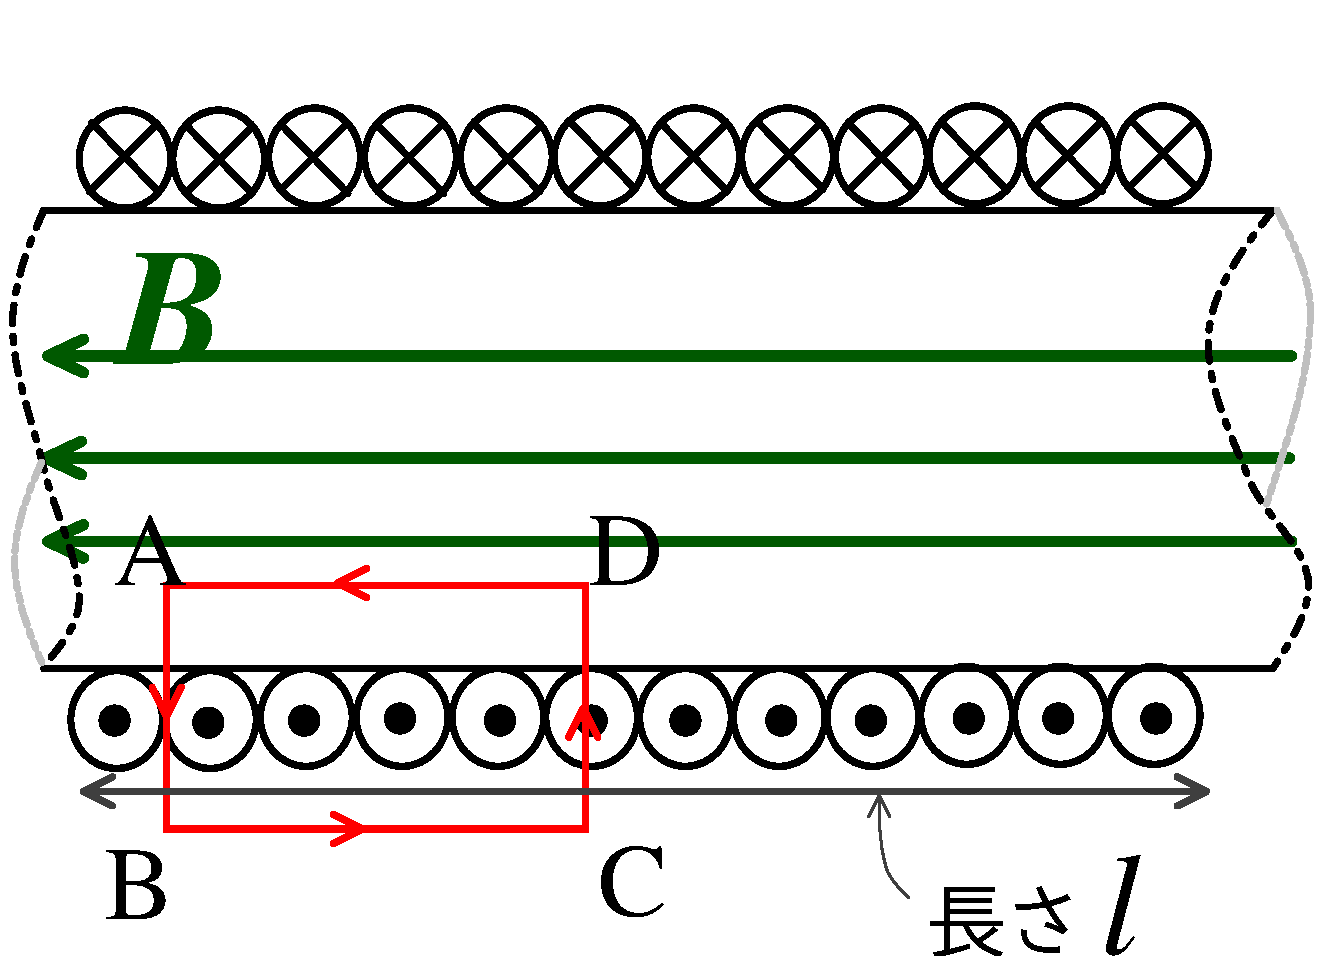
\includegraphics[keepaspectratio, width=3.5cm,height=2.8cm,clip]{sorenoido22.pdf}
                            \caption{ソレノイド(内部)}
                            \label{fig:sorenoido22}
                        \end{center}
                        \end{minipage}
                    \end{tabular}
                \end{figure}

        いま,ソレノイドを流れる電流 $I$ が定常状態であるとしたとき,アンペールの法則によって
        1回巻きの場合
        \begin{align}
            \oint_{l}B\,\df l =\mu_{0}I
        \end{align}
        である.$l$ はアンペールの法則に依れば任意の閉曲線
        であるから,ここでは図\ref{fig:sorenoido22}のように閉曲線をとってみる.閉曲線ABCDで,
        辺AB,辺CDの方向には,電流と平行な向きであるので,磁束密度は現れない.
        また,閉曲線ABCDの辺BCの部分には磁束密度は存在しない.なぜなら,この辺BCの部分は磁束密度が
        存在しない無限遠方と同じ空間でなければならないからである.つまり,
        磁束はソレノイドの内部だけに存在することになる.
        \begin{equation*}
            \oint_{l}B\,\df l=Bl
        \end{equation*}
        と計算されるから,
        \begin{align}
            Bl=\mu_{0} I.
        \end{align}
        $N$ 回巻きの場合は,これを $N$ 倍すればよく,
        \begin{align}\label{sorenoidoB}
            Bl=N\mu_{0} I \\ \notag
            \therefore\quad B=\frac{N\mu_{0} I}{l}
        \end{align}
        この式(\ref{sorenoidoB})がソレノイド状のコイルに流れる電流がつくる磁束密度である.従って,
        この磁束密度を磁束 $\Phi$ に代入すると,
            \begin{align}
                \Phi_{l}=\frac{NS\mu_{0} I}{l}
            \end{align}
        である.
            \begin{myshadebox}{ソレノイドコイルの自己インダクタンス}
                ソレノイドコイルの自己インダクタンス $L$ は,以下の式で表される.
                \begin{align}
                    L := \frac{NS\mu_{0}}{l}.
                \end{align}
                $N$ はコイルの巻数,$S$ はコイルの断面積,$l$ はコイルの長さである.
            \end{myshadebox}
        \end{memo}


%======================================================================
%  Section
%======================================================================
    \section{電子回路の構成要素}
    %==================================================================
    % Subsection
    %==================================================================
    \subsection{ダイオード}
        \subsubsection{ダイオードとは}
        電流を一方向しか流さないようにする素子が存在する.
        この素子に生じる電流は,いうなれば一方通行であり,
        逆向きに電流を通すことはしない.このような動きを
        する素子を,\textbf{ダイオード} という.

        \subsubsection{ダイオードの回路図記号}
            ダイオードの回路図記号は図\ref{fig:kairozu_Diode}の通り.
            矢印の方向が正方向である.逆向きに電流は流さない.
            \begin{figure}[hbt]
                \begin{center}
                    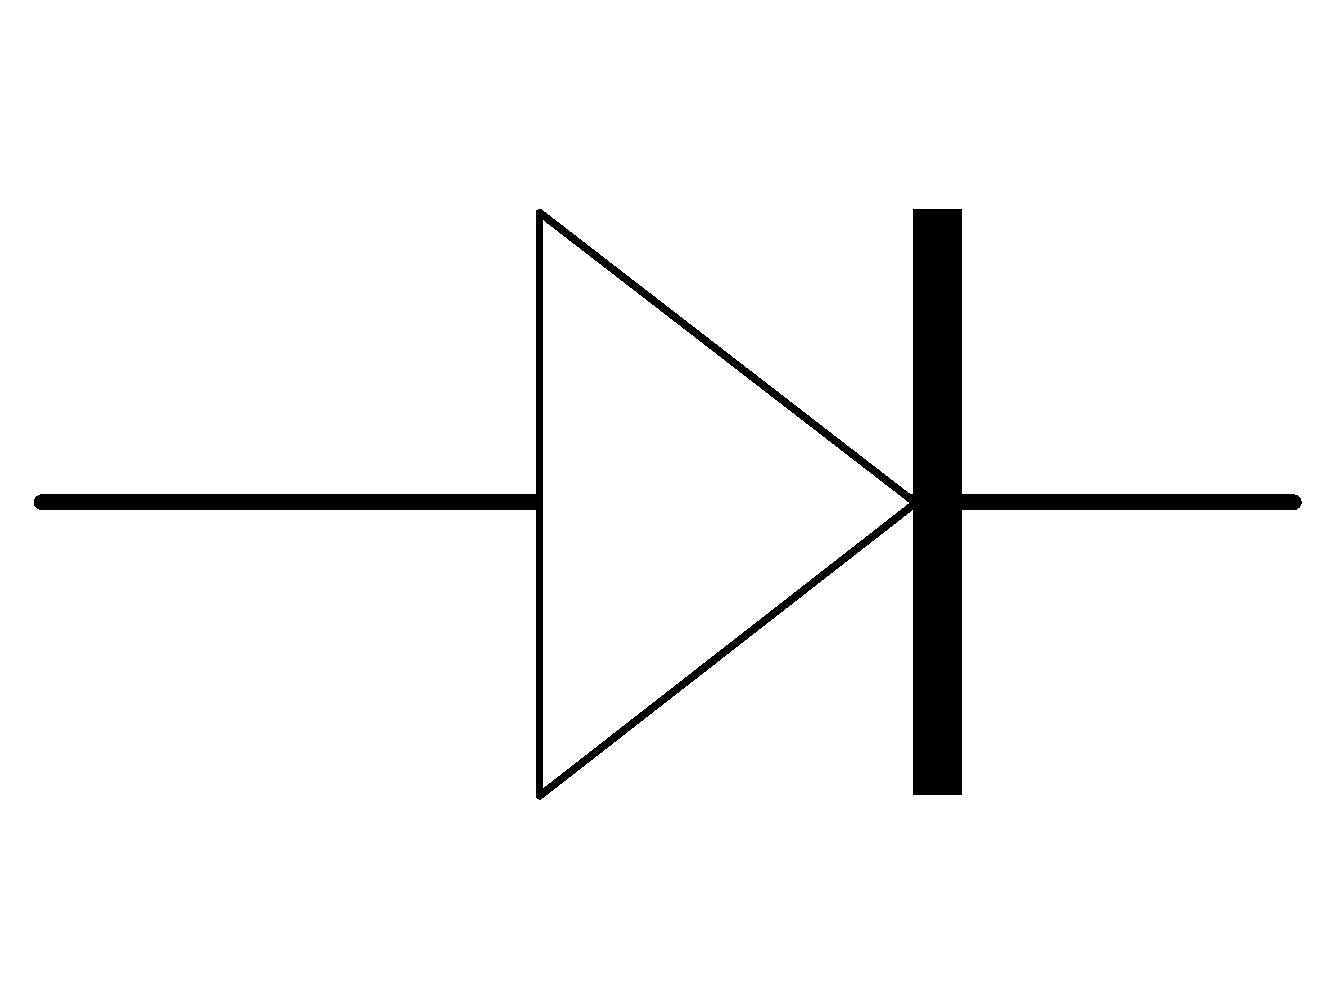
\includegraphics[keepaspectratio, width=2cm,height=1.5cm,clip]{kairozu_Diode.pdf}
                    \caption{ダイオードの回路図記号}
                    \label{fig:kairozu_Diode}
                \end{center}
            \end{figure}

        ダイオードはどのように構成されるかといった説明は後回し
        にして,ここではそのような素子が存在することを知っても
        らうだけでよい.

        \subsubsection{ダイオードの特性}
        ダイオードを用いた最も簡単な電子回路を図\ref{fig:Diode_Tokusei}に示す.
        電子回路の理論で仮定されている理想的なダイオードには,抵抗がない.
        抵抗を挟んでいる理由はこのためであり,電圧源のショートを抑える働きを
        する.

        ダイオードの両端には,電源電圧によって,電圧がかかっているが,負方向に
        電圧がかかっても,その方向には電流は流さない.これを象徴的に図にしたのが,
        図\ref{fig:Diode_Tokusei}である.
                \begin{figure}[hbt]
                    \begin{tabular}{cc}
                        \begin{minipage}{0.5\hsize}
                            \begin{center}
                                \includegraphicsdouble{Diode_kairo.pdf}
                                \caption{ダイオードを用いた電子回路}
                                \label{fig:Diode_kairo}
                            \end{center}
                        \end{minipage}
                        \begin{minipage}{0.5\hsize}
                            \begin{center}
                                \includegraphicsdouble{Diode_Tokusei.pdf}
                                \caption{ダイオードの動作}
                                \label{fig:Diode_Tokusei}
                            \end{center}
                        \end{minipage}
                    \end{tabular}
                \end{figure}

    %==================================================================
    % Subsection
    %==================================================================
    \subsection{トランジスタ}

    %==================================================================
    % Subsection
    %==================================================================
    \subsection{受動的な素子/能動的な素子}
        今までの素子(抵抗,キャパシタ,インダクタ)と違い,
        ダイオードやトランジスタは,
        自身におかれた条件(端子の電位差)によりその特性を変える.ここで,
        特性といったのは,一方方向にしか電流を流さないということである.
        このように,素子の両端にかかる電圧と,素子に生じる電流により,その
        特性を変えるものを,\textbf{能動的}な素子という.

        また,抵抗$\cdots$キャパシタ$\cdots$インダクタの3つ素子は,
        電流や電圧の向きにより,その特性を変化させることはない.
        このような素子は,周囲の状況に流されるといったイメージで,
        \textbf{受動的}な素子といわれる.

        \begin{memo}{回路が「記憶」できるようになった}
            ダイオードやトランジスタ
            の,能動的な性質により,電子回路に「記憶」という仕組み
                \footnote{
                    LSI(集積回路)で言うところの,フリップフロップ$\cdot$ラッチのこと.
                    コンピュータ(CPU)では,レジスタやメモリがその例として挙げれる.
                }
            を実現することが可能になった
                \footnote{
                    どのように実現するのかについて,後ほど簡単に触れてみたい.
                }.

            このおかげで,今日私たちはパソコンや携帯電話などの電子機器を活用し,
            便利な生活を送ることができるのである.
        \end{memo}

%======================================================================
%  Section
%======================================================================
    \section{電磁気学とのつながり}
        \begin{mycomment}
            電気回路で起こる現象は,物理法則---特に電磁気学,
            マクスウェル方程式---に従っている.
            そこで,ここでは,抵抗/キャパシタンス/自己インダクタンスは
            物理的にどのように説明されるのかを,紹介しておこう.
            実際に電気回路を作る時には,いちいち意識しないことであるが,
            基本的な知識(常識/教養的な意味で)として,知っておいたほうが良い.
        \end{mycomment}

        \subsection{コンダクタンス}
        物体には,電流が生じやすいものと電流が生じにくいものに
        大まかに分類できるが,そのための指標がないと,
        数式的に表現できず,つまりは回路解析ができない.
        そこで,ここでは,物体の電流の生じやすさの指標を導入する.

        物体の電流の生じやすさの指標の名前は,\textbf{コンダクタンス} と
        よばれる.ここで,簡単な実験を考える.何か物体が目の前にあるとしよう.
        そして,この物体の電流の生じやすさを知りたいとする.この場合,
        適当な電圧をその物体に与え,その時に生じる電流を測定することが,
        電流の生じさを把握する上で最も適した方法である.
        この実験を,ひとつの物体だけでなく,複数種類の物体に対して行うと,
        次のような電流と電圧の関係を得られる.\\
            \begin{itembox}[l]{電流の生じやすさ}
                多くの物体
                    \footnote{
                        “すべての物体ではない”ことに注意.
                    }
                で,以下の関係が成立している.すなわち,物体のある2点を特定し,
                その2点に対して電圧 $V$ を与えて,その時の電流値 $I$ を測定すると,
                $V$ と $I$ には比例関係が成立している.この比例定数を $G$ で表す.
                すると,電圧と電流の関係は,次式で表せる.
                    \begin{align}
                        V = GI.
                    \end{align}
            \end{itembox}

            上の式を比例定数 $G$ について解く.
                \begin{equation*}
                    G = \frac{I}{V}.
                \end{equation*}
            こうすることで,“電圧に対する電流”がイメージしやすくなった.
            この式を見れば,低い電圧で大電流が生じれば,当然,コンダクタンス $G$ は
            大きくなる.ということは,電流が生じやすいということを,数値的に表現
            できたことになる.よって,この比例定数であるコンダクタンスこそが,
            物体の電流の生じやすさの指標として,定義できる.
            \begin{myshadebox}{コンダクタンス}
                \textbf{コンダクタンス} は,
                物体の電流の生じやすさの指標であり,次式で定義される量である.
                    \begin{align}
                        G := \frac{I}{V}.
                    \end{align}
                ここに,$I$ は物体に生じる電流であり,
                $V$ は物体の2点間にかける電圧である.
            \end{myshadebox}

                ただし,例えば,タングステンや半導体など,
                電流と電圧が比例関係を満たさない物体も存在する.
                その場合は,コンダクタンスは上式で定義されない.
                ただし,電流と電圧には関数関係は成立していて,
                局所的にはコンダクタンスを定義することは可能である
                    \footnote{
                        つまり,電位 $V$ を微小変化させたときには,
                        電流 $I$ は比例しているとみなして,微分で
                        コンダクタンスを定義するのである.
                            \begin{align}
                                G := \frac{\rd I}{\rd V}.
                            \end{align}
                    }.
                ただし,このノートの電気回路の部分では,このような特殊な性質をもつ
                物体は考慮しない.対象とする物体の性質として,電流が電圧に比例する
                ようなものを考えることとする.

                また,この比例関係は実験的に得られるものであり,
                その実験の際には,温度の変化はないという,暗黙の
                仮定もその定義の内に含まれていることに注意しよう.

        \subsection{抵抗}
            電流の生じやすさを表す指標をコンダクタンスと定義した.さらに,
            今度は逆に,電流の生じにくさを表す指標を考える.といっても,
            さらに新しい量を導入するわけではない.電流の生じにくさを表すには,
            ご存知,抵抗を使えば良い.抵抗は,コンダクタンスの逆数として定義
            される.抵抗を表す文字を $R$ とすると,定義は次のようになる.
            \begin{myshadebox}{抵抗}
                \textbf{抵抗} は,物体の電流の生じにくさ指標であり,
                コンダクタンスの逆数として,次式で定義される量である.
                    \begin{align}\label{eq:teikouno_teigisiki}
                        R := \frac{1}{G} = \frac{1}{I/V}= \frac{V}{I}.
                    \end{align}
                ここに,$I$ は物体に生じる電流であり,
                $V$ は物体の2点間にかける電圧である.
            \end{myshadebox}

            抵抗は,コンダクタンスをもとに定義したりょうであり,つまり,
            コンダクタンスが定義できない物質
                \footnote{
                    半導体,タングステンなど.
                }
            に対しては,抵抗も定義できない.

        \subsection{オームの法則}
            上の抵抗の定義式(\ref{eq:teikouno_teigisiki})より,電圧 $V$ に
            ついて解けば,よく知られている,\textbf{オームの法則} の式になる.
                \begin{align}
                    V = RI.
                \end{align}
            この式は,エネルギー保存則に従っている.次のように式変形してみよう.
                \begin{align}
                    V +(- RI) = 0.
                \end{align}
            この式で,$V$ は外から与らえるている起電力(外部起電力)である.
            そして,$-RI$ は何を意味するかというと,回路内に起こる電位の変化
            を意味している.負の記号が付いているので,回路内で電位が下がることが
            示されている
                \footnote{
                    わざわざ,括弧をつけてまで,負の記号を強調したのは,
                    その合計(和)が0になるということを,しめすためである.
                }.
            \begin{myshadebox}{オームの法則}
                ある物体に起電力を与えたとき,その物体内部にはその起電力の向きに
                逆向きな電位差が生じる.そして,外部起電力と物体に生じる電位差の
                合計は0になる.物体の抵抗値を $R$ とし,物体にかける電圧を $V$,
                その時に生じる電流を $I$ とすれば,\textbf{オームの法則} は
                    \begin{align}
                        V +(- RI) = 0
                    \end{align}
                と表現できる.$V$ が外部起電力であり,$(-RI)$ が物体に生じる電位差である.
            \end{myshadebox}

            オームの法則は,電圧と電流と抵抗の3つの概念の関係式であり,
            定義式ではない.よく,$V=RI$ と書いてしまうから,中学生の頃には,
            この式で,抵抗が定義されるのだと思い込んでしまっていた
                \footnote{
                    速度の定義式 $v=x/t$ と同じように考えてしまったのである.
                }
            しかし,あくまでも,オームの法則は単なる関係式である.何かを定義している
            訳ではない
                \footnote{
                    このノートでは,コンダクタンスを電流と電圧で定義し,その基礎としているが,
                    実を言うと,この定義も説明のための便宜的なものであり,コンダクタンスの定義
                    式も関係式なのである.
                }.
            電気回路論におけるオームの法則は,ニュートン力学でいうと運動方程式に対応する.
            ニュートンの運動方程式も,質量 $m$ と 力 $\bF$,加速度 $\df^{2} \br/\df t^{2}$ の
            関係式
                \begin{equation*}
                    m \frac{\df^{2} \br}{\df t^{2}} = \bF
                \end{equation*}
            にすぎず,これで力 $\bF$ を定義しているわけでも,加速度 $\df^{2} \br/\df t^{2}$ を
            定義しているわけでもない.


        \subsection{オームの法則は物理法則ではない}
            オームの法則は“法則”とよばれているが,実は,一般的に成立するような
            ものではない.つまり,オームの法則に従わない材料も存在するのである
            その代表的なものに半導体やタングステンが紹介されることが多い.また,
            大概の金属は常温ではオームの法則に従うが,高温環境になるとオームの法則は
            成り立たなくなる.

            とはいっても,オームの法則は電気回路の基本法則である.
            電気回路が使われるのはほとんどの場合が常温であり,
            オームの法則に従う材料を導線として使えば回路設計も簡単だからだ.
            特殊な材料を使わなければならないとか,高温環境で使用される場合で,
            オームの法則に従わないことが考えられる場合でも,基本的な考え方は同じ.
            オームの法則からずれる部分を実験で測ったり,理論的に計算したりして差分を吸収する
            ように調整することで,問題解決できる.
            電気回路が使用される環境は,多くの場合,材料がオームの法則に従うと考えてよい
            \footnote{
                オームの法則に従わない材料を導線として使うこともあるのかもしれないが,
                私にはそのようなことが要求される場面を想像できない.万が一あるとしても,
                たいへん特殊な場合であろう.
            },
            だから,オームの法則は回路設計や動作解析の際に重宝される.実際,電気回路の理論の
            根幹をなす法則は,このオームの法則と,キルヒホフの電流則と同電流則の3つだけである.
            これをもとにして数学的に解析できてしまうのだ
            \footnote{
                電気回路を論ずる際に使用される数学は,線形代数と微分方程式である.
                計算を楽にする単に技術的なものとして,複素関数論が使われることもある.
                具体的には,フーリエ級数,フーリエ変換,ラプラス変換だ.
                電気回路や電子回路で多用される数学理論は,電気数学と総称される.
            }.

            オームの法則は物理法則ではないというからには,物理法則から導出できるはずである.
            次節では,オームの法則の導出を見ていくが,実は,導き方が複数考えられる.
            このノートでは,有名な3つの導出方法を考える.

        \subsection{オームの法則の導出1:高校生への標準的な説明}
            電気抵抗が生じるのはなぜか.もう少し詳しく考える
                \footnote{
                    とはいっても,
                    量子力学の知識がないので,少し理想化しすぎな部分があるが,
                    そこら辺は無視しよう.詳細は「物性」関係の教科書を参照するとよい.
                }.
            物体は原子によって構成されるが,この原子はさらに細かく見ると,電子と原子核
            によって構成されている.
            とりあえずは,ここまでの知識でよい
                \footnote{
                    さらにいえば,原子核は陽子や中性子で構成されることや,さらに陽子や
                    中性子は
                    クォークによって構成されていることがわかっているが,ここではこんな
                    ことを考えてもしょうがない.
                }.

            導体には,\textbf{自由電子} とよばれる,原子核よりも少し離れた電子がある.
            この電子は原子核に束縛されることなく,自由に導体内を移動できる-----自由と
            入っても,
            導体の外に勝手に出て行くことはないが.

            導体の例として,銅線(導線ではない!!)を考える.もちろん,他の導体でも同様
            の議論ができるがイメージしやすいようにするためにそうする.

            銅線にだって小さいとはいえど抵抗がある.抵抗が生じる原因は,電子が移動の際
            に,原子核と衝突することである.「電流とは電子の移動のことである」というこ
            とはJ. J. トムソンらの実験によってわかっている.
            原子を構成するのは電子と原子核だが,電子は原子核の1800倍も小さく,電子の移
            動の際には,原子核は静止していると考えても差し支えない.もっと正確にいうと原子核は完全
            に静止しているのではなく,その場で振動している.この振動が電子との衝突を生むのである.電子の移動が原
            子核によって妨げられるということで
            ,それが抵抗という現象となって現れるのである.

            定量的に考えてみよう.まずは,微分方程式を使わないずに,高校レベルで考える.

            ここに,長さ$l$[m],面積 $S$[m${}^{2}$] の銅線があるとする.
            この銅線の単位体積(1[m${}^{3}$])あたり
            の電子の個数を $n$ としよう.この $n$ は銅線中の電子の単位体積あたりの密度
            を表している.
            電子の電荷を $-e$ とおこう.
            電子は銅線中を移動している.銅線中の電子はたくさんある.
            もちろん,複数の電子が全く同じ速さをもって移動しているわけでは
            なく,ここの電子は気まぐれに様々な速度で移動している.そこで,この速さの平均を
            考えることにし,これを $\bar{v}$ と表現する.今仮に,
            速度 $\bar{v}$ の一定速度で動く電子を考える.
                        \begin{figure}[hbt]
                            \begin{center}
                                \includegraphicslarge{o-munohousoku.pdf}
                                \label{fig:o-munohousoku}
                                \caption{オームの法則}
                            \end{center}
                        \end{figure}

            電流 $I$ は単位時間(1秒)あたりに,正電荷がどれだけ通過したかによって
            表せる
                \footnote{
                    電子が負の電荷をもっているのは,電流の定義の方が電子の発見よりも
                    早い時期になされたからである.正電荷は,特に何もしなければ,
                    電位の高いほうから低いほうへと移動する.電流はこのような正電荷を
                    仮定して定義していた.しかし,実験によって電子が発見されたとき,電子は
                    電位の低い方から高いほうへと移動した.だから電子はマイナスの電荷をも
                    っているのである.

                    慣習上,電流の向きの定義を逆にし直すことはないようである.
                    電流の向きの定義を逆にするには労力が必要であるし,
                    それをおこなっても,大した利点がないからだろう.
                }.
            電流とは電子の移動であるから,
                \begin{align}\label{eq:teikou_1}
                    I=(-e)n\bar{v}S
                \end{align}
            と書ける.

            ところで,電子はクーロン力 $-eE$ を受ける.
            さらに電子は,速度 $\bar{v}$ で運動する際に,原子核から受ける抵抗 $k\bar{v}$ を受ける.
            この $k$ は定数である.ここでは原子核から受ける抵抗は速度に比例すると
            近似している.電子が銅線中を一定の速度 $\bar{v}$ で動いているので,
            クーロン力と原子核から受ける抵抗力は釣り合っているはずである.つまり,
                \begin{align}\label{teikou_2}
                    -eE=k\bar{v}
                \end{align}
            が成立している.

            さらに,銅線の両端部分の電位差のことを \textbf{電位} というが,
            この電位は[銅線内の電場]と[銅線の長さ]の積で表される.なぜなら,
            電位は単位電荷が電場からなされる仕事として定義されているのである.
            単位電荷は1[C]の電気量をもつ電荷であり,従って,これは電場 $E$ より
            受けるクーロン力も $E$ である.単位電荷が電場 $E$ によって $l$ だけ変位したのならば,
            単位電荷が電場 $E$ より受けた仕事は $lE$ ということになる.
            銅線の両端の電圧を $V$ と表せば,
                \begin{align}\label{teikou_3}
                    V=lE
                \end{align}
            と書ける.

            以上の3つの式(\ref{eq:teikou_1}),(\ref{teikou_2}),(\ref{teikou_3})より,
            オームの法則を導いてみよう.まず,式(\ref{teikou_2})の両辺に $l$ をかける.
                \begin{align*}
                    -eEl=k\bar{v}l
                \end{align*}
            この式の左辺は,式(\ref{teikou_3})から $V=El$ だから,
                \begin{align*}
                    -eV&=k\bar{v}l \notag \\
                    \Leftrightarrow \quad \bar{v}&=-\frac{eV}{kl}
                \end{align*}
            この $\bar{v}$ を式(\ref{eq:teikou_1})に代入する.
                \begin{align*}
                    I&=(-e)n\left(-\frac{eV}{kl}\right) S \notag \\
                    \Leftrightarrow \quad I&=\frac{ne^{2}}{k}\frac{S}{l}V
                \end{align*}
            これを $V$ について解くと,
                \begin{align}
                    V=\frac{k}{ne^{2}}\frac{l}{S}I
                \end{align}
            である.右辺の $I$ 以外は全て定数である
                \footnote{
                    面積 $S$ と長さ $l$ は実験で測定できる.
                }.
            この定数が抵抗を表している.
                \begin{align}
                    R=\frac{k}{ne^{2}}\frac{l}{S}
                \end{align}
            以上から,オームの法則
                \begin{align}
                    V=RI
                \end{align}
            が求まった.

        \subsection{オームの法則の導出2: 微分方程式}
            導出の雰囲気をつかんだところで,微分方程式を用いてもう少し具体的に
            オームの法則を導出してみよう.まず,電流の根源は電子の運動であるから,
            この電子の運動方程式をたてる.

            起電力により導体内に電場 $E$ が
            あるはずで,電子はこの電場からクーロン力$eE$を受けている.
            さらに,
            導体中の電子は陽イオン(原子核のこと)にぶつかりながら運動する.
            もちろん,衝突の際には速度は変化する.これを平均して $v_{d}$ と表現する.
            これは,電子が図\ref{fig:11dff}のように,導体内をヨロヨロしながら運動するためで,
            このような電子の動きをドリフトしているという.
            この $v_{d}$ のことを \textbf{ドリフト速度} という.
                \begin{figure}[hbt]
                    \begin{center}
                        \includegraphicsdefault{dft.pdf}
                        \label{fig:11dff}
                        \caption{電子のドリフト}
                    \end{center}
                \end{figure}

            このように電子は陽イオンから抵抗力を受けながら導体内を運動するわけだが,
            この抵抗力は電子のドリフト速度に比例していると仮定してよいとするなら,
            適当にその係数を用意し,これを $k$ として,抵抗力を $-kv_{d}$ とする.
            抵抗力に負符号がつくのは,ドリフト速度と逆向きだからである.以上を踏まえて,
            電子の質量を $m_{e}$ とすれば,電子の運動方程式は
                \begin{align}\label{eq:ohms_law_diveq_model1}
                    m_{e}\frac{\df v_{d}}{\df t}=-eE-kv_{d}
                \end{align}
            である.この電子の運動方程式を解いていこう.まず,両辺を $m_{e}$ で割る.
                \begin{align}
                    \frac{\df v_{d}}{\df t}=-\frac{eE}{m_{e}}-\frac{k}{m_{e}}v_{d}
                \end{align}
            次に,少しトリッキーではあるが,右辺を $-k/m_{e}$ でくくる.
                \begin{align}\label{eequ}
                    \frac{\df v_{d}}{\df t}=-\frac{k}{m_{e}}\left(v_{d}+\frac{m_{e}}{k}\frac{eE}{m_{e}}\right)
                \end{align}
            この式の右辺の括弧の中を $\xi $ とおく.
                \begin{align}\label{1234}
                    \xi := v_{d}+\frac{m_{e}}{k}\frac{eE}{m_{e}}
                \end{align}
            この $\xi$ を時間 $t$ で微分して
                \begin{align}\label{4321}
                    \frac{\df \xi}{\df t}=\frac{\df }{\df t}\left(v_{d}+\frac{m_{e}}{k}\frac{eE}{m_{e}}\right) =\frac{\df v_{d}}{\df t}
                \end{align}
            である.

            式(\ref{1234})と式(\ref{4321})を式(\ref{eequ})に考慮すれば,
                \begin{align}\label{QQQ}
                    \frac{\df \xi}{\df t}=-\frac{k}{m_{e}}\xi
                \end{align}
            という方程式となる.
            この微分方程式を解いてみよう.ここでは,計算の細かい部分は多少省略する
                \footnote{
                    ここでの式変形は,$\df t$ 等を1つの数のようにみなして計算する事がある.
                    このような計算ができることは,微分方程式の教科書を参照して確認して欲しい.
                }.
            まず,$\df \xi$ と $\df t$ を1つの独立な数のように扱い,以下のように変形する.
                \begin{equation*}
                    \frac{1}{\xi}\df\xi = - \frac{k}{m_{e}}\df t
                \end{equation*}
            これは,$\df \xi$ に関する項と $\df t$ に関する項を,それぞれ左辺と右辺にまとめたものである.
            次に両辺を不定積分する.このとき,左辺は $\df \xi$ で積分し,右辺は $\df t$ で積分する.
                \begin{equation*}
                    \frac{1}{\xi}\df \xi = - \frac{k}{m_{e}}\df t
                    \quad\Leftrightarrow\quad
                    \int\frac{1}{\xi}\df \xi = - \int\frac{k}{m_{e}}\df t
                \end{equation*}
                \begin{equation*}
                    \Leftrightarrow\quad
                    \log\xi = -\frac{k}{m_{e}}t + C
                    \quad\Leftrightarrow\quad
                    \quad\xi = \e^{-\frac{k}{m_{e}}t+C} = \e^{-\frac{k}{m_{e}}t}\e^{C}
                \end{equation*}
                \begin{equation*}
                    \therefore\quad
                    \xi = A\e^{-\frac{k}{m_{e}}t}\,,\quad ( A = \e^{C})
                \end{equation*}

            解が上のように求まった.$\xi$   は式(\ref{1234})で定義された量
            であることを思い起こせば,
                \begin{equation*}
                    A e^{-\frac{k}{m_{e}}t}=v_{d}+\frac{m_{e}}{k}\frac{eE}{m_{e}}
                \end{equation*}
            である.これを $v_{d}$ について解いて
                \begin{align}
                    v_{d}=A e^{-\frac{k}{m_{e}}t} - \frac{eE}{k}
                \end{align}
            となる.

            もともと知りたかったのは,多数の電子の運動が平均して安定している状況における解である.
            安定な状態とは,導体に起電力が与えられてから,
            十分に時間が経過したときのことである($t\rightarrow \infty$)
            \footnote{
                十分に時間がたてば安定状態に至るという,暗黙の仮定がなされている.
                これまで得た知識からでは,この暗黙の仮定の妥当性を示せない.
                ここでは,時間がたつと安定状態になるという経験をもとに,この仮定の正当性を主張する.
            }
            第一項は0になって,
                \begin{equation*}
                    v_{d}=-\frac{eE}{k}
                \end{equation*}
            となる
            \footnote{
                第一項が0になることを確認しておこう.
                \begin{equation*}
                    \lim_{t \to \infty} e^{-\frac{k}{m_{e}}t} = e^{- \infty} = \frac{1}{e^{\infty}}=\frac{1}{\infty} = 0.
                \end{equation*}
            }.これが導線内の自由電子のドリフト速度であり,\textbf{終速度} ともいわれる.

            ところで,以前,式(\ref{eq:teikou_1}) において,電流 $I=-en\bar{v}S$ と表せることを認めた.
            これに表れる平均の速度 $\bar{v}$ は,終速度 $v_{d}$ と同一視することができて,
                \begin{equation*}
                    I = -en\left( -\frac{eE}{k} \right)S = \frac{e^{2}nE}{k}S.
                \end{equation*}

            さらに,電圧 $V$ と電場 $E$ の関係は,距離 $d$ を比例定数として,$V=dE$ が成立していることは,
            前に確認済みである
            \footnote{
                電場に関するガウスの法則での具体例として,よく取り上げられる問題であり,電磁気学と電気回路
                を繋ぐ大切な式である.
            }.
            この距離 $d$ は,ここでは導線の長さ $l$ に相当する
            \footnote{
                導線の形が直線であると暗に仮定してしまったが,これは計算を簡単にするための便宜上の仮定である,
                導線が曲がっていたら,線積分を考えればいい.曲がっている場合を想定しても数学的な議論が可能
                だけれど,得られる結果は直線を想定した場合とほとんど変わりはなく,議論が面倒になるだけだ.
                \begin{equation*}
                    V = \oint_{C} \bE \cdot \df \bl \quad , \quad \mbox{$C$ : 導線の形}.
                \end{equation*}
            }
            から $V=lE$ である.これを $E$ について解いて $E=V/l$.これを上の式に代入すると,
                \begin{equation*}
                    I = \frac{e^{2}nE}{k}S = \frac{e^{2}n(V/l)}{k}S = \frac{e^{2}nV}{k}\frac{S}{l}.
                \end{equation*}
            これを $V$ について解くと
                \begin{align}
                    V = \frac{k}{e^{2}n}\frac{l}{S}I
                \end{align}
            となって,一番目に求めたオームの法則の式と同じ式がえられた.

            ついでに,定数 $k$ について,もう少し踏み込んでみよう.
            定数 $k$ は,電子のドリフト速度 $v_{d}$ と,そのときの
            陽イオンから受ける抵抗力の比例定数として使ってきたが,もう少し詳細を見てみよう.といっても,
            最初に立てた微分方程式(\ref{eq:ohms_law_diveq_model1})を次元解析をするだけ.
            式(\ref{eq:ohms_law_diveq_model1})見ると,定数 $k$ の次元は [kg/s] であることが要請されている
            \footnote{
                以下の次元解析を行う.次の微分方程式
                \begin{equation*}
                    m_{e}\frac{\df v_{d}}{\df t}=-eE-kv_{d}
                \end{equation*}
                の次元を見ると,[kg][m/s][s${}^{-1}$]=[C][V/m]+[X][m/s] である.
                左辺の[s${}^{-1}$] は,時間 $t$ に関する微分によるものである.
                [X] が今知りたい $k$ の次元だ.
                とりあえず,[X] を含む第二項を考えると,[kg][m/s][s${}^{-1}$]=[X][m/s] であり,[X] について
                解いて整理すると,[X]=[kg/s] を得る.第一項については,今の考察には関係ないので,省略する.
                電流と力の関係や電場(電位)の定義に立ち返れば,同じ次元をもつことが確認できるだろう.
            }.
            よって,$\tau$ を静止状態の電子が終速度までに達するまでの時間としたとき,
            \begin{equation*}
                k=\frac{m_{e}}{\tau}
            \end{equation*}
            とできる
            \footnote{
                $k$ を $\tau$ に書き換えただけなので,論理的には何の進展もない.しかし,
                なんだかわからない定数だった $k$ が少し具体的に見えたことに意義がある.
            }.
            $\tau$ の物理的な意味は,「電子が陽イオンに衝突してから次の衝突までの時間」である.
            言い換えれば,電子は時間 $\tau$ の間は何にも衝突せず,自由に動き回っている時間であることから,
            この $\tau$ を \textbf{平均自由時間} という
            \footnote{
                ちなみに,平均自由時間 $\tau$ の間に電子が移動する距離を,
                \textbf{平均自由行程} という.
            }.
            そうすると,終速度 $v_{d}$ は
                \begin{align}
                    v_{d}= \frac{eE}{(m_{e}/\tau)}=\frac{eE\tau}{m_{e}}
                \end{align}
            となる.

            最後に,定数部分を抵抗 $R$ として,
                \begin{equation*}
                    R := \frac{m_{e}}{e^{2}n\tau}\frac{l}{S}
                \end{equation*}
            を定義すれば,
                \begin{equation*}
                    V=RI
                \end{equation*}
            が導かれる.

                        \begin{figure}[hbt]
                            \begin{center}
                                \includegraphicslarge{hjj.pdf}
                                \label{fig:hjj}
                                \caption{平均自由時間}
                            \end{center}
                        \end{figure}

        \subsection{オームの法則の導出3:電子移動度}
            先ほど,電子は導線の原子にぶつかりながら,導線中を移動すると
            説明し,このような電子がもつ速度のことを,\textbf{ドリフト速度} と
            いうと書いた.ここで,ドリフト速度をもう少し詳しく考えてみよう.
            ただし,ここでの電子の運動は,古典的な粒子を想定する
                \footnote{
                    電子は,量子力学においては,単なる粒子ではなく,
                    波動の性質も同時に備えもつ.しかしここでは,電子を
                    単純な粒子であると仮定し,話を進めていくことにする.
                }.

            電子が原子にぶつかってから,他の原子にぶつかる直前までの過程を
            考える.導線中を運動している電子が,導体を構成する原子に
            衝突したとき,電子の速度は0になると考える.そしてその後,
            電子は徐々に加速し,また,原子にぶつかる.
                    \begin{figure}[hbt]
                        \begin{center}
                            \includegraphicslarge{drift_sokudo.pdf}
                            \label{fig:drift_sokudo}
                            \caption{電子移動度・電子緩和時間}
                        \end{center}
                    \end{figure}

            電子は電場から常にクーロン力を受けており,加速度運動をしている.
            衝突直後から,次の衝突の直前までの間に,電子の移動距離 $d$ は
            どの程度かを計算してみよう.

            ニュートン力学において,等加速度運動における位置の公式を
            計算したことがある.結果を以下に書き下そう.
                \begin{equation*}
                    x(t) = \frac{1}{2} a t^{2}  +  v_{0}t + x_{0}
                \end{equation*}
            ここに,$a$ は加速度である.
            また,$v_{0}$,$x_{0}$ は初期値である.今回は0であるとして考える.
            初速度は,衝突直後は
            完全に速度は0になると仮定し,0とする.すると,
                \begin{equation*}
                    x(t) = \frac{1}{2} a t^{2}
                \end{equation*}
            のみが残る.今回は,電子の原子との衝突から他原子の衝突までの
            時間を考えているので,$t=T - t_{0}$ とすればよい.$t_{0}$ は現在の時刻である.
            しかし,話を簡単にするために,$t_{0} = 0$ として考える.つまり,$t = T$ とする.
                \begin{equation*}
                    x(T) = d = \frac{1}{2} a T^{2}
                \end{equation*}

            ところで,電子は,回路内の電場 $E$ より,クーロン力 $F$ を受けている.これは,
            クーロンの法則で,
                \begin{equation*}
                    F = -eE
                \end{equation*}
            と書かれる.ここに,$-e$ は電子のもつ電荷量である.
            この時の,電子の運動方程式
                \footnote{
                    ニュートンの運動方程式は,力 $\bF$,加速度 $\ba$,質量 $m$ の関係を表し,
                        \begin{equation*}
                            m\ba = \bF
                        \end{equation*}
                    と書かれる.
                }
            は次のようになる.
                \begin{equation*}
                    ma  =  -eE.
                \end{equation*}
            これにより,電子の加速度を得る.すなわち,
                \begin{equation*}
                    a  =  -\frac{eE}{m}.
                \end{equation*}

            これを,先ほどの等加速度運動の公式に代入してみよう.
                \begin{equation*}
                    d = -\frac{1}{2} \frac{eE}{m} T^{2}
                \end{equation*}
            という式を得る.この式の時間 $t$ は,電子が原子と衝突してから,
            別の原子と衝突するまでの時間である.

            導体中を移動する
            電子の平均の速度 $v_{e}$ を考えてみよう.平均の速度 $v_{e}$ とは,この場合,
            電子の運動を等速直線運動とみなして,計算することと同じである.
            等速直線運動では,位置 $x$ は $x = v_{0}t$ という関係式が成立
            している.速度について解けば,$v_{0} = x/t$ である.
            つまり,平均の速度を知りたければ,位置を時間で割ってやればよい.
            すると,
                \begin{equation*}
                    v_{e}  =  -\frac{d}{T} = -\frac{1}{2} \frac{eE}{m} T
                \end{equation*}
            となる.この式で,$e$ は電子のもつ電荷量,$m$ は電子の
            質量であるので,これらは,定数である.これを意識して,
            式を書き変えてみよう.
                \begin{equation*}
                    v_{e}  =   -\frac{T}{2} \frac{e}{m}E.
                \end{equation*}
            さらに,$T/2$ も,電子の衝突の周期によるもので,
            これらは平均して一定であると仮定して,
                \begin{align}
                    \tau := \frac{T}{2}
                \end{align}
            とおく.この $\tau$ を \textbf{電子緩和時間} とよぶ.
            すると,平均の速度の式は次のように表現される.
                \begin{equation*}
                    v_{e}   =  -\frac{e\tau}{m} E
                \end{equation*}
            さて,速度は,上の式より,電場 $E$ に比例することが明らかになった.
            その依存関係は,比例定数によって決まる.そこで,この比例定数は,
            \textbf{電子移動度} という名前でよばれる.
                \begin{align}
                    \mu_{e} =  \frac{e\tau}{m}
                \end{align}
            で表される.この $\mu_{e}$ は,電磁気学で用いた透磁率の記号と同じであるが,
            それとは全く関係のない概念であることに,注意すべきだ.

            以上により,電子が導線中を移動する平均の速度を求めることができた.
            その式は,
                \begin{align}
                    v_{e} =  -\mu_{e}E
                \end{align}
            で表される.
            マイナスが付いているのは,今考えている電荷が電子であることによる.
            電子の電荷量が負だからである.もちろん,正の電荷量をもつと仮定すれば,
            マイナスの符号は付かない.

            この式により,電子のドリフト速度は,
            導体内の電場に比例することが分かる.

        \subsection{ジュール熱と電力}
            電気回路に起電力をつなぐと,実際には抵抗部分に熱を生じることはよく知っているだろう.
            この熱は \textbf{ジュール熱} よばれている.なぜ,ジュール熱が発生するのだろうか.

            電池をつないでから,電流が生じるまでを考えてみよう.もちろん,電池接続された直接の結果
            が電流の発生ではない.電池が電気回路の両端に接続されると,電池の両端には電位差があるから,
            その電位差が電気回路内部に発生する.これは電気回路内部に電場が生じることを意味する.電場の伝わ
            る速さは,前章で確認したように,光速 $c = 3\times 10^{8}$[m/s] である.この電場によっ
            て,導線にある自由電子がクーロン力を受けて,運動を始める.この電子の運動が,電流である.
            電子は力を受け続けると,速度はどんどん上がってしまうが,電気回路内部では自由電子の
            速度は,どのようになっているのだろうか.前項目で考えたように,運動する自由電子は,導線
            を構成する原子核にぶつかって速度を落とす.自由電子は導線内に多数存在するが,それらを平
            均すると,一定の速度に落ち着く.これを終端速度ということを前項目で確認した.自由電子が
            原子核にぶつかったとき,原子核は電子の運動量を受ける.この電子から受け取った運動量によ
            り,原子核は運動しようとする.しかし,電子から受け取る運動量は,原子核をその場から移動
            させるほどの大きさではない.原子核はその衝突前の位置を中心に,振動する.この原子核の振
            動を,私達は熱として感じるのである.1つの電子の原子核の衝突では,微々たるものだが,自
            由電子や原子核は導線中に多数存在することを考えれば,納得がいくだろう.
                        \begin{figure}[hbt]
                            \begin{center}
                                \includegraphicslarge{denryoku.pdf}
                                \label{fig:denryoku}
                                \caption{電子と原子核の衝突}
                            \end{center}
                        \end{figure}

            数量的に考えてみよう.起電力 $V_{l}$ と電場 $E$ の関係は,
                \begin{equation*}
                    V_{l} = \oint_{l} E \df l = lE
                \end{equation*}
            である
                \footnote{
                    $V_{l}$ の添え字 $l$ 電気回路の閉ループ(loop)の頭文字 $l$ を意識してつけた.
                }.
            ここでは電場は電気回路内で一定(電池内部は除く)とし,電気回路の長さを $l$ であるとした.
            この起電力 $V_{l}$ が1つの電荷(ここでは電子)にする仕事を考える.言い方を変えれば,
            電子が起電力から得るエネルギーを考えることと同じである.
            電位の定義は,単位電荷が受ける仕事として定義されているので,電子の電荷を $q_{e}$ と
            書くことにすれば,電子が起電力から受け取るエネルギー $\flwE$ は,
                \begin{equation*}
                    \flwE = q_{e}V_{l}
                \end{equation*}
            である
                \footnote{
                    エネルギーの記号に $E$ ではなく, $\flwE$ を用いた理由は,
                    電場の $E$ と区別するためである.ニュートン力学ではエネルギーを表す記号として $E$ が
                    使われることが多いが,電磁気学での $E$ は電場の強さを意味することが一般的である.
                    このように,物理学では,同一の記号を全く違う物理的対象に当てることが多い.
                    アルファベットが26文字しかないので,このようのことはよく起こる.記号が何を
                    意味して用いられているかは,常に注意をしながら式を読む必要がある.

                    別の例だと,この後に確認するが,自己インダクタンスの記号として,$L$ が用いられる
                    が,これは角運動量とは全く別の概念である.
                }.
            実際には,電荷は運動していて,これが電流 $I_{l}$ だから,$I_{l}=\df q_{e}/\df t$ である
                \footnote{
                    $l$ は,起電力 $V_{l}$ と統一するため,
                    同様に電気回路の閉ループ(loop)の頭文字を意識してつけた.
                }.
            上式で,電荷 $q_{e}$ を電流に置き換えたいので,両辺を時間微分しよう.すると,
                \begin{equation*}
                    \frac{\df \flwE}{\df t} = \frac{\df q_{e}}{\df t}V_{l}=I_{l}V_{l}
                \end{equation*}
            となって,電流 $I_{l}$ を式に取り入れることができた.
            再び両辺を時間積分しよう.すると
                \begin{equation*}
                    \int \frac{\df \flwE}{\df t} \df t   =   \int I_{l}V_{l} \df t
                \end{equation*}
            であるが,起電力(電圧)と電流はともに時間変化しない定数であると仮定し,
                \begin{equation*}
                    \flwE = I_{l}V_{l}t
                \end{equation*}
            である.これが起電力が導線中の電子に与えるエネルギーである.特に $t = 1$ として,
            単位時間中に,起電力が電気回路に与えるエネルギーとして,\textbf{電力} $P$ が定義される.

            起電力が導線にエネルギーを与えることを,改めて実感したことだろう.
            つまり,熱の原因は,この電力にあるということである.
                \begin{myshadebox}{電力の定義}
                    単位時間中に,起電力が電気回路に与えるエネルギーを \textbf{電力} と
                    いい,ここでは記号 $P$ を用いて表すことにする.電力 $P$ と電流 $I$ と
                    電圧 $V$ の間には,以下の関係式が成立する.
                        \begin{align}
                            P:= IV.
                        \end{align}
                    オームの法則 $V=RI$ を考慮すれば,電力 $P$ は
                    次のように表現することも可能である.
                        \begin{align}
                            P= IV = RI^{2} = \frac{V^{2}}{R}.
                        \end{align}
                \end{myshadebox}

        \subsection{電流と電球の発光との関係}
            電気回路につながれた電球がある.
            導線に電池をつなぐと,電流が生じる.実際にこれを確かめるには,抵抗と電球を
            直列につなぎ,そしてその両端に電池をつなげる.電球が光ることから,この電気回路
            に電流が流れたことが,目で見て確認できる.
               \begin{figure}[hbt]
                   \begin{center}
                       \includegraphicslarge{kidenryoku_to_denryu.pdf}
                       \label{fig:kidenryoku_to_denryu}
                       \caption{電流が流れたかな?}
                   \end{center}
               \end{figure}

            ここで,少し疑問になる事がある.それは,「なぜ,電球が光ったら,その電気回路に電流が流れて
            いると言えるのか」ということである.電気回路に電流が流れていないのに,電球が光ることはない
            のか.また,電気回路に電流が流れているけれども,電球が光らないことはないのか.

            この問題は,電球を構成する物質について考える必要がある.

        \subsection{電気抵抗率}\label{subsub:teikou_ritu}
            前項目で抵抗の式,つまり,
                \begin{align}
                    R=\frac{k}{ne^{2}}\frac{l}{S}
                \end{align}
            が導出されたついでに,抵抗率についても考えておこう.
            式を見ればわかるように,抵抗は導線(銅線ではない!!)の
            長さ $l$ に比例し断面積 $S$ に
            反比例する.ということは,
            抵抗を長さ $l$ と断面積 $S$ の一種の関数のように見ることができる.
            で,この関数の定数部分に注目して,これを \textbf{電気抵抗率} という.
            単に \textbf{抵抗率} といってしまうことのほうが多い.抵抗率は
            普通,$\rho$ で表現される.つまり,
                \begin{align}
                    \rho=\frac{k}{ne^{2}}
                \end{align}
            である.

            しかし通常,抵抗率という場合には,この式の右辺はあまり意識しない.
            何らかの定数であることには変わりないが,
            この定数は実験的に直接的に測定されてしまうことが多い.
            右辺の $k/ne^{2}$ は大した
            意味がないように思われる.

            抵抗率を使えば,抵抗は
                \begin{align}
                    R=\rho\frac{l}{S}
                \end{align}
            と書かれる.

            \subsection{電気伝導率}
            抵抗率の逆数 $1/\rho$ を \textbf{電気伝導率} といい,$\sigma$ で
            表す.抵抗率と同様に,単に \textbf{伝導率} ということも多い.つまり,
                \begin{align}
                    \sigma=\frac{1}{\rho}
                \end{align}
            である.

            導線は,その抵抗率が大きいほど,電流を通しにくくなる.これを逆手に考えれば,
            つまり,抵抗率が小さいほど,電流を通しやすくなるということになる.電気伝導率とは,
            式の等号の意味において,
            抵抗と同じ意味をもつのだけども,着眼点が少し異なっていることに
            注意したい.

            電気伝導率を使うと,電流密度 $\bi$ と電場 $\bE$ に関係させて,
            オームの法則は次のようにも表現できる.
            \begin{align}
                i=\sigma E.
            \end{align}

            なぜなら,
            \begin{align*}
                V &= RI=\rho\frac{l}{S}I=\frac{1}{\sigma}\frac{l}{S}I \\
                \Leftrightarrow \quad
                \sigma V &= \frac{l}{S}I.
            \end{align*}
            ここで,電流と電流密度の関係式
            \begin{equation*}
                I = \sint_{S} \bi \cdot \bn \df S
            \end{equation*}
            から
                \footnote{
                    $S$ は曲面,
                    $\df S$ は曲面 $S$ の微小部分,
                    $\bn$ は $\df S$ の単位法線ベクトル.
                },
            \begin{equation*}
                \sigma V = \frac{l}{S}\sint_{S} \bi \cdot \bn \df S
            \end{equation*}
            さらに,電場 $\bE$ と電位差 $V$ の関係式
            \begin{equation*}
                V=\int_{l} \bE \cdot \bt \df \l.
            \end{equation*}
            より
                \footnote{
                    $l$ は線積分の任意の経路(導線にほかならない),
                    $\df l$ は $l$ の微小部分,
                    $\bt$ は $\df l$ の単位接線ベクトル.

                },
            \begin{align*}
                     \sigma \int_{l} \bE \cdot \bt \df \l
                &=  \frac{l}{S}\sint_{S} \bi \cdot \bn \df S. \\
                \Leftrightarrow \quad
                     \sigma \int_{l} |\bE||\bt| \cos\theta \df l
                &=  \frac{l}{S}\sint_{S} |\bi||\bn|\cos\theta \df l \\
                     \sigma \int_{l} E\df l
                &=  \frac{l}{S}\sint_{S} i \df S \\
                     \sigma E  \int_{l} \df l
                &=  \frac{l}{S}i\sint_{S} \df S \\
                     \sigma  El
                &=  \frac{l}{S}iS \\
                \therefore \quad
                \sigma E &= i
            \end{align*}
            計算途中,$|\bt|=1$,$|\bn|=1$,$\theta=\pi/2$ であることに注意しよう.
                \begin{figure}[hbt]
                    \begin{center}
                        \includegraphicsdefault{OhmSlaw_IsigmaE.pdf}
                        \label{fig:OhmSlaw_IsigmaE}
                        \caption{オームの法則を拡張する($\bi=\sigma\bE$)}
                    \end{center}
                \end{figure}

        \subsubsection{キャパシタンスの形と容量の関係}
        キャパシタンスは,形によって容量が変化する.形と容量の関係は,
        数式的に表現できる.ここでそれを確認しておこう.
        キャパシタンスの両端には電圧がかかっており,十分に時間が
        経っていて,電荷が十分に溜まっているとする.
                    \begin{figure}[hbt]
                        \begin{center}
                            \includegraphicsdefault{capacita_youryou.pdf}
                            \label{fig:capacita_youryou}
                            \caption{キャパシタンスの形と容量}
                        \end{center}
                    \end{figure}

        キャパシタンスの形を,各電極間の距離を $d$,電極の面積を $S$ とする.ガウスの法則を
        使って,一方の電極から生じている電場の強さを求めてみよう.電場の向きは,キャパシ
        タンスに垂直であると考える.ここでは,その大きさのみを考える.とりあえず,ガウスの
        法則を書いてみよう.その形式は,計算が楽な積分形を用意しよう.キャパシタンスの一方の電極を含むよ
        うに,図の点線で囲ったように,閉曲面をとる.この閉曲面を $A$ とする
            \footnote{
                閉曲面はど
                のような形にしても,ガウスの法則は成立するので,計算のしやすさを考えてとる
                べきだ.今回の場合は,電極平面から平行な電場の成分はないことから,円柱
                型の閉曲面をとることにした.こうすることで,側面から流れ出る電場を考慮する
                必要がなくなって,計算が楽になるからである.
            }.
        このとき,ガウスの法則の積分形は
            \begin{equation*}
                \varepsilon_{0}\int_{S_{A}}\bE
                \cdot\textit{\textbf{n}}\df S_{A}
                =\int_{\Omega_{S_{A}}} \rho\df V_{A}
            \end{equation*}
        と書ける.
        $S_{A}$ と $V_{A}$ の添字の $A$ はそれぞれ,閉曲面 $A$ の表面積,体積を意識して
        書いた.円柱の閉曲面 $A$ は上面 $At$ (t:top),側面 $As$ (s:side),下面 $Ab$ (b:bottom) の3部分に
        分けて考える($A=At+As+Ab$).

        右辺と左辺を別々に計算していこう.まず,左辺を考える.
            \begin{align*}
            \mbox{[左辺]}  &= \varepsilon_{0} \int_{S_{A}}  E\df S_{A} \\
                           &= \varepsilon_{0}
                                \left(
                                    \int_{S_{At}} E_{\perp}\df     S_{At} +
                                    \int_{S_{As}} E_{\parallel}\df S_{As} +
                                    \int_{S_{Ab}} E_{\perp}\df     S_{Ab}
                                \right)
            \end{align*}
        であるが,電極に平行な電場成分 $E_{\parallel}$ は 0 だから,第2項はなくなり,
            \begin{align*}
            \mbox{[左辺]}      = \varepsilon_{0}
                                    \left(
                                        \int_{S_{At}}E_{\perp}\df S_{At} +
                                        \int_{S_{Ab}}E_{\perp}\df S_{Ab}
                                    \right)
            \end{align*}
        さらに,電極の一方に生じる電荷量は,他方の電荷量の反対符号である.
        つまり,一方の電極から生じる電場は全て,他方の電極に吸収される.
        これは,キャパシタンスの外部には電場の漏れがないことを意味している.
        従って,今回の場合,キャパシタンスの外部に電場を生じるような向き
        の,閉曲面 $A$ の上面からは電場は生じていないことになる.よって,
        式はさらに簡単になる.
            \begin{align*}
            \mbox{[左辺]}  = \varepsilon_{0}\int_{S_{Ab}}E_{\perp}\df S_{Ab}
                    = \varepsilon_{0} E_{\perp} S_{Ab}
            \end{align*}
        以下,$E_{\perp}$,$S_{Ab}$ の添字はいつでも同じになるので,添字を省略して記述する.
            \begin{equation*}
            \mbox{[左辺]}  = \varepsilon_{0} E S_{A}.
            \end{equation*}
        キャパシタンス全体で考えれば $S_{A} = S$ であり,
            \begin{align}
                \mbox{[左辺]}  = \varepsilon_{0} E S.
            \end{align}

        次に,ガウスの法則の右辺を考える.電荷密度は,総電荷をその面積で割ったものである.
        今回,キャパシタンスにたまっている電荷は $Q$ だから,
            \begin{align}
                \mbox{[右辺]} = \int_{\Omega_{A}} \rho\df V_{A} = Q.
            \end{align}

        以上から,\mbox{[左辺]}$=$[右辺] をとすれば,
            \begin{equation*}
                \varepsilon_{0} ES = Q
            \end{equation*}
        となり,これより,キャパシタンス内部の電場 $E$ は
            \begin{align}
                E = \frac{Q}{\varepsilon_{0}S}
            \end{align}
        を得る.これから,キャパシタンスの両端の電位差を計算できる.
        電場と電位差の関係は
            \begin{equation*}
                V = \oint_{l} E \df l
            \end{equation*}
        である.今回,経路 $l$ はキャパシタンスの距離にとればよく,その長さは $d$ である.
        つまり,
            \begin{equation*}
                V = E \oint_{l} \df l = Ed
            \end{equation*}
        これに求めたキャパシタンス内の電場 $E = Q/\varepsilon_{0}S$ を代入することで,
            \begin{align}
                V = \frac{Q}{\varepsilon_{0}S}d
                \quad\Leftrightarrow\quad
                \frac{Q}{V} = \varepsilon_{0}\frac{S}{d}
            \end{align}
        を得る.

        ここで,キャパシタンスの要領の定義式 $C = Q/V$ を考慮すれば,
            \begin{align}
                C = \varepsilon_{0}\frac{S}{d}
            \end{align}
        を得る.
            \begin{myshadebox}{キャパシタンスの形状と容量の関係}
                キャパシタンス $C$ と形状の関係は次のようである.
                    \begin{align}
                        C:=\frac{Q}{V} = \varepsilon_{0}\frac{S}{d}
                    \end{align}
                ここに,
                        $Q$ はキャパシタンスに溜まる電気量,
                        $V$ はその時のキャパシタンスの両端の電位差,
                        $\varepsilon_{0}$ は真空の誘電率,
                        $S$ はキャパシタンスの断面積
                        $d$ はキャパシタンスを構成する導体板間の距離
                である.
            \end{myshadebox}

        \begin{memo}{電気力線と等電位線は直交する}
            電荷が,無限に広い平面に,一様に分布しているとき,この平面から生じている
            電場はどのようになっているかをここで確認する.結論からいえば,このとき,
            平面に垂直な方向に電場が生じているのである.これは,導体の表面は等電位である
            ことと,電場と電位の関係
                \footnote{
                    電気力線と,等電位線は垂直に交わる.
                }
            を考えれば,すんなりと説明できる.この説明は電磁気学の部分で行っているので,
            今回は,別の方法で,説明してみよう.

            まず,平面
            上に任意の点をとり,これを点Aとしよう.この点Aを通るように,図のような円
            を描く.この円の上に,点Aとその円の中心を通る直線上に,点Bをとる.これら
            点Aと点Bのそれぞれの部分の電荷密度がつくる電場を合成すると,図に示したよ
            うに,平面に平行な電場の成分は相殺されて,正味0となる.つまり,平面に平
            行な電場はないということである.よって,電場は平面に垂直な成分のみが残り,
            これが,平面に分布した電荷密度のつくる電場となる.
                        \begin{figure}[hbt]
                            \begin{center}
                                \includegraphicsdefault{capacita_denba.pdf}
                                \label{fig:capacita_denba}
                                \caption{無限平面上に分布した電荷密度より生じる電場}
                            \end{center}
                        \end{figure}

            もちろん,今の場合,無限に広い平面に電荷密度が分布しているとしたので,
            平面の端は存在しないから,平面上のどの部分を見ても,面に垂直な電場が
            生じている.しかし,実際には,平面は有限であるので,その平面の端砲で
            は対称性がなく,電場が歪む.有限の場合でも,その平面の中心付近では
            無限平面と同様に考えられるので,このノートでは平面の端の部分について
            は,考慮しないことにして,話を簡略化する.
        \end{memo}




%===================================================================================================
%  Chapter : 代表的な電気回路
%  説明    : 電気回路の例を上げて,その動作を解析する.
%               ・抵抗のみの回路
%               ・インダクタと抵抗の回路(直列)
%               ・キャパシタと抵抗の回路(直列)
%               ・抵抗,インダクタ,キャパシタの直列回路
%               ・インダクタと抵抗の回路(並列)
%               ・キャパシタと抵抗の回路(並列)
%               ・抵抗,インダクタ,キャパシタの並列回路
%               ・積分回路
%               ・微分回路
%               ・変圧器
%            について,記述する
%===================================================================================================
\chapter{代表的な電気回路}
%   %-----------------------------------------------------------------------------------------------
%   %  Input
%   %    File Name : PhysNote_EECircuit_Ecirc00.tex
%   %    説明      : 電磁気学を構成する基本的な概念を説明する.
%   %-----------------------------------------------------------------------------------------------
        %===================================================================================================
%  Chapter : 代表的な電気回路
%  説明    : 電気回路の例を上げて,その動作を解析する
%===================================================================================================

%======================================================================
%  Section
%======================================================================
    \section{抵抗のみの回路}
    \section{インダクタと抵抗の回路(直列)}
    \section{キャパシタと抵抗の回路(直列)}
    \section{抵抗,インダクタ,キャパシタの直列回路}
    \section{インダクタと抵抗の回路(並列)}
    \section{キャパシタと抵抗の回路(並列)}
    \section{抵抗,インダクタ,キャパシタの並列回路}
    \section{積分回路}
    \section{微分回路}
    \section{変圧器}



%===================================================================================================
%  Chapter : 代表的な電子回路
%  説明    : 電気回路の例を上げて,その動作を解析する.
%               ・整流回路(インバータ)
%               ・増幅回路
%            について,記述する
%===================================================================================================
\chapter{代表的な電子回路}
%   %-----------------------------------------------------------------------------------------------
%   %  Input
%   %    File Name : PhysNote_EECircuit_Ecirc01.tex
%   %    説明      : 電子回路の例を挙げ,その動作の解析を行う
%   %-----------------------------------------------------------------------------------------------
        %===================================================================================================
%  Chapter : 代表的な電子回路
%  説明    : 電気回路の例を上げて,その動作を解析する.
%===================================================================================================

%======================================================================
%  Section
%======================================================================
    \section{整流回路(インバータ)}

%======================================================================
%  Section
%======================================================================
    \section{増幅回路}
    %==================================================================
    % SubSection
    %==================================================================
    \subsection{「増幅」の意味}


%===================================================================================================
%  Chapter : コンピュータの物理学的基礎
%  説明    : コンピュータの動作を,電磁気学に立ち返って説明する
%===================================================================================================
\chapter{コンピュータの物理学的基礎}
%   %-----------------------------------------------------------------------------------------------
%   %  Input
%   %    File Name : PhysNote_EECircuit_CompPrim.tex
%   %    説明      : 電子回路の例を挙げ,その動作の解析を行う
%   %-----------------------------------------------------------------------------------------------
        %===================================================================================================
%  Chapter : コンピュータの物理学的基礎
%  説明    : コンピュータの動作を,電磁気学に立ち返って説明する
%===================================================================================================

%======================================================================
%  Section
%======================================================================
    \section{考え方と方針}
    ここでは,大規模な電子回路である,コンピュータについて考える.
    一般論として,電子計算機を学ぶのも1つの方法であるが,
    このノートでは現実性を重視し,実際のコンピュータが電子回路によって,
    構成可能かどうかを検証することとしたい
        \footnote{
            「コンピュータが電子回路によって構成買うであることを“検証”したい」
            と書いたが,現実にコンピュータが存在しているので,すでに検証済みである
            と考えられるだろう.その通りである.しかし,今の私にはコンピュータが
            本当に電子回路の知識で構成可能かどうかは理解していない.わかっているのは,
            コンピュータが存在している事実であって,コンピュータが電子回路であるという
            ことはわかっているわけではない.なので,この章で
            コンピュータの動作原理を理解し,コンピュータが電子回路で構成可能である
            ということを確認したいと思う.

            しかし,コンピュータの動作原理を説明する教科書には,
            物理学的な基礎から書かれているものがない
            (見当たらない).しかし,確かに,コンピュータは現実に存在し
            ていて,\textbf{コンピュータは物理法則に則って動作している}はずである.そこで,
            コンピュータの動きを,物理法則から理解できるということを文書にまとめ,
            知識を整理することで理解を深めていきたいと思う.
         }.
    以降の議論はかなり荒削り
        \footnote{
            壊滅的に等しい.
        }
    だが,コンピュータがどのように物理法則に則って計算を行っているか,
    というイメージをもつのには十分であると思う.

    あくまでも,\textbf{目的は,コンピュータが物理法則に従って計算を行なっている
    ということを“実感すること”}である.

    \begin{memo}{注意}
        説明のために,簡易的なコンピュータを(頭の中で)つくることになるが,
        あくまでも私が考えた構成のもので,現実的なものではない.それは,上記の
        目的
            \footnote{
                目的:「コンピュータがどのように物理法則に則って計算を行っているか」
                というイメージをもつこと.
            }
        のためにつくるものであって,実際のコンピュータがそうなっているの
        ではない.「ああ,たしかに,こうやって構成すれば,コンピュータが
        作れるんだな」という感覚を抱けるようになりたいのだ.
    \end{memo}


%======================================================================
%  Section
%======================================================================
    \section{電磁気学の復習}
    \begin{mycomment}
        まずは,基礎中の基礎の確認から始めよう.
    \end{mycomment}
    %==================================================================
    % SubSection
    %==================================================================
    \subsection{電子の存在}
    \textbf{電子} がないと,電磁気現象は生じない.もともと,電磁気現象の
    根源として,\textbf{電荷} の存在が仮定(要請)されていて,これをもとに
    電磁気学が構成されている.電磁気学が成立した後,存在を仮定していた
    電荷というものが,電子という形で実在することが,実験により確かめられた.
    しかし,電子のもつ電気量は,電磁気学で定める正電気量の反対の符号を
    もつことも確かめられた.そうは言っても,電子が電磁気現象の根源
    であることは,今では,絶対に否定できない事実である.

    コンピュータも電子回路のひとつである以上,電子の存在の上に成り立って
    いるものである.コンピュータ内部の回路を移動する電子こそが,計算の動力
    源となるだ.

    %==================================================================
    % SubSection
    %==================================================================
    \subsection{「ホール(hole)」という考え方}
    \textbf{ホール} という語彙は,正確には,
    \textbf{エレクトロン$\cdot$ホール(Electron hole)} と
    いう.また,日本語に訳して,\textbf{正孔} とも言われる
        \footnote{
            正孔:「せいこう」と読む.
        }.
    このノートでは,「ホール」という言い方を採用する.次に,肝心のホールとは
    何かを,説明しよう.

    ホールとは,簡単に言えば,電子の抜け殻とでも表現できよう.
    元々電子が存在すべき場所なのだが,実際には電子が存在しない部分を,
    ホールと呼んでいる.
       \begin{figure}[hbt]
           \begin{tabular}{cc}
               \begin{minipage}{0.5\hsize}
                   \begin{center}
                       \includegraphicsdouble{Comp_ElecHole_EleMov.pdf}

                       (A)
                   \end{center}
               \end{minipage}
               \begin{minipage}{0.5\hsize}
                   \begin{center}
                       \includegraphicsdouble{Comp_ElecHole_EleMov01.pdf}

                       (B)
                   \end{center}
               \end{minipage}
           \end{tabular}
       \end{figure}
       \begin{figure}[hbt]
           \begin{tabular}{cc}
               \begin{minipage}{0.5\hsize}
                   \begin{center}
                       \includegraphicsdouble{Comp_ElecHole_EleMov02.pdf}

                       (C)
                   \end{center}
               \end{minipage}
               \begin{minipage}{0.5\hsize}
                   \begin{center}
                       \includegraphicsdouble{Comp_ElecHole_EleMov03.pdf}

                        (D)
                   \end{center}
               \end{minipage}
           \end{tabular}
           \caption{ホールの動き(実際は電子の動き)}
       \end{figure}


    なんで,こんなこと(ホール)を考える必要があるのか.
    結論から言えば,実はホールという概念は絶対に必要というわけではない.
    しかし,ホールという考え方を用いることにより,物理的イメージが
    捉えやすくなり,物理現象の説明も短くなり簡潔にまとめることができるのだ.
    だったら,これを採用しない手はない.

    \begin{memo}{炭酸の泡 --- ホールに似た現象として ---}
        似たような考え方の例として,炭酸飲料の気泡がよく挙げられる.
        この気泡が,ホールに対応するのである.たんさんの入っていない
        飲み物には,当然,泡は生じない
            \footnote{
                もちろん,振ったり,ストローか何かで内部に気体(空気)を
                入れれば泡ができるが,ここでは理想的(液体に対してなんの操作もしていない)
                な状態を想定している.
            }.
        しかし,炭酸飲料の場合には,内部から泡が生じる.これは,圧力により
        液体に溶けていた二酸化炭素などの気体が,圧力の低下に伴って,外部に
        出ようとして泡として現れるものである.
        このとき,本来ならば液体が存在する場所なのだが,実際には泡(気体)が
        眼に見えてくる.そして,この泡は液体中を,上に向かって移動する.いや,
        この言い方は,正確ではない.なぜなら,こう表現してしまうと,気体が
        重力に逆らっているように,捉えられてしまうからである.では,本当の
        ところは,どう説明すればよいのだろうか.答えは,視点を変えることである.
        泡を見るのではなく,液体を見るのである.つまり,液体が気体の下に潜り込む
        ように落ちるのである.

        現象の流れは次のように説明できる.最初の段階では,炭酸飲料には圧力
        がかけられていて,気体は内部に溶けたままである
            \footnote{
                炭酸飲料が入ったペットボトルが未開封の状態に相当する.
            }.
        そして,炭酸飲料にかける圧力を低くする
            \footnote{
                ペットボトルのフタを開ける.
            }.
        すると,液体の内部から気体が生じてくる
            \footnote{
                圧力によって,液体中に抑えつけられるように閉じ込められていた気体が,
                圧力を緩めたことによって,泡となって液体中から飛び出してくる.
            }.
        一度液体中から気体が生じれば,液体は気体より重いので,液体は気体の下の方へ
        入り込もうとする
            \footnote{
                泡に視点を合わせれば,泡は上へ移動していくように見える.
            }.
        この結果として,泡が上に移動しているように見えるのだ.屁理屈を言っている
        ような気がするが
            \footnote{
                日常会話でこんなことを説明したら,屁理以外の何ものでも
                ないだろう.
            },
        正確さを求める場合には,高説明するしかない(と思う).
    \end{memo}

    %==================================================================
    % SubSection
    %==================================================================
    \subsection{電荷保存則}
        %==============================================================
        % SubsubSection
        %==============================================================
        \subsubsection{電場に対するガウスの法則}
            \begin{align}
                \ddiv \bE = \frac{1}{\varepsilon_{0}}\rho.
            \end{align}

        %==============================================================
        % SubsubSection
        %==============================================================
        \subsubsection{アンペール$=$マクスウェルの法則}
            \begin{align}
                \drot \bB = \mu_{0}\bi + \varepsilon_{0}\mu_{0}\frac{\rd \bE}{\rd t}.
            \end{align}

        %==============================================================
        % SubsubSection
        %==============================================================
        \subsubsection{電荷保存の法則}

    %==================================================================
    % SubSection
    %==================================================================
    \subsection{電位(電圧)の定義}

%======================================================================
%  Section
%======================================================================
    \section{トランジスタの動作概要}
    %==================================================================
    % SubSection
    %==================================================================
    \subsection{半導体}
        %==============================================================
        % SubsubSection
        %==============================================================
        \subsubsection{半導体の分類}
        \begin{figure}[hbt]
            \begin{center}
                \includegraphicslarge{handoutai_bunrui.pdf}
                \caption{半導体の分類}
                \label{fig:handoutai_bunrui2}
            \end{center}
        \end{figure}

        %==============================================================
        % SubsubSection
        %==============================================================
        \subsubsection{真性半導体}

        %==============================================================
        % SubsubSection
        %==============================================================
        \subsubsection{n型半導体,ドナー}

        %==============================================================
        % SubsubSection
        %==============================================================
        \subsubsection{p型半導体,アクセプタ}

    %==================================================================
    % SubSection
    %==================================================================
    \subsection{ダイオード}

    %==================================================================
    % SubSection
    %==================================================================
    \subsection{ダイオードの電流電圧特性}

    %==================================================================
    % SubSection
    %==================================================================
    \subsection{トランジスタの物理構成}
        %==============================================================
        % SubsubSection
        %==============================================================
        \subsubsection{バイポーラトランジスタの物理構成}

        %==============================================================
        % SubsubSection
        %==============================================================
        \subsubsection{電界効果型トランジスタ(FET)の物理構成}

        %==============================================================
        % SubsubSection
        %==============================================================
        \subsubsection{MOSFETトランジスタ(MIS構造)の物理構成}

        %==============================================================
        % SubsubSection
        %==============================================================
        \subsubsection{CMOSの物理構成}

    %==================================================================
    % SubSection
    %==================================================================
    \subsection{トランジスタの動作}
        %==============================================================
        % SubsubSection
        %==============================================================
        \subsubsection{バイポーラトランジスタの動作原理}
        電流により,電流の増幅率を調整する.

        %==============================================================
        % SubsubSection
        %==============================================================
        \subsubsection{MOSFETトランジスタ(MIS構造)の物理構成}
        電圧により,電流の増幅率を調整する.

        %==============================================================
        % SubsubSection
        %==============================================================
        \subsubsection{トランジスタの動作(これだけを覚えていれば十分)}


%======================================================================
%  Section
%======================================================================
    \section{コンピュータの構成概要}
    \begin{mycomment}
        「コンピュータの構成」は現実のところ,様々である.
        それは開発される回路の数だけ存在するからである.
        同じ回路を開発するのは,骨折り損だ.しかし,
        コンピュータの構成の思想はどれも同じである.
        それは,「命令」による「データ加工」である.
    \end{mycomment}

    %==================================================================
    % SubSection
    %==================================================================
    \subsection{コンピュータの定義}
        %==============================================================
        % SubsubSection
        %==============================================================
        \subsubsection{コンピュータとは何か}
            まず始めに,明確にして置かなければならないことがある.それは,
                \begin{center}
                    「コンピュータとは何か.」
                \end{center}
            ということだ.何を今更,と思うかもしれないが,
            いざこの質問に答えようとすると,曖昧になってしまうのではなかろうか.
            この質問の答えとして,例えば,電気関係にうとい一般の方だとしたら,
            「何かものすごい計算を行うもの」だとかと答えそうである.
            また,普段仕事でパソコンを使っている人には,
            「MicrosoftのWordやExcelなど
            で文書を作成したり,表計算をするをするものである」という
            答が返ってきそうでもある.これらの答えは,大きな枠組みの範囲では
            正しい.しかし,これから議論していくには,コンピュータの定義
            としては,不十分である.では,どのように定義したらよいのだろうか.

            一般的に,コンピュータを定義することは難しい.これは
            「世界初のコンピュータは誰が開発したか」という質問に対して,
            パスカル

            だとか,
            バベッジ

            だとかと言われるように,複数の解答が寄せられることにも,
            定義の難しさ,あるいは認識の曖昧さが現れている.
            この違いは,コンピュータをどう定義の違いの現れなのだ.
            答えとして,誰を上げても,間違いはない
                \footnote{
                    もちろん,コンピュータを自分なりに定義して,
                    それを最初に創り上げた人で無いといけない.
                }.
            パスカルは四則演算を機械的に行える装置を作ったし,
            ライプニッツはそれを改良して桁上がりにも対応させた.
            さらに,バベッジはプログラムと言う概念をその計算機に折込み,
            自動で計算を行えるような装置を考案した
                \footnote{
                    実際に装置が作られたのは,彼の死後である.
                    ただ,文書として理論が残されており,これを基に
                    後の人々がその理論の正しさを実証している.
                }.

            このように,コンピュータを単なる四則演算器として捉えるならば,
            パスカルがその創始者となる.しかし,私の知る限りでは,
            コンピュータの定義として,「計算を自動的に行うもの」と
            されることが多く,その意味では,計算をプログラム制御によって
            自動化することに成功した,バベッジがその答えとされることが
            多いと感じている.

            このノートでは,コンピュータを次のように定義し,以降では,この定義を基にして話を進めていく.
                \begin{myshadebox}{(このノートの)コンピュータの定義}
                    \textbf{コンピュータ} とは,\textbf{命令} による \textbf{データ} の \textbf{加工} を
                    自動で行う装置である.
                \end{myshadebox}

            「命令」,「データ」,「加工」の定義については,後ほど詳しく
            記述することとしたいが,さしあたっては,次のように捉えておいて欲しい.
            命令とは,「四則演算を行え」ということであり,データはその四則演算の
            対象となる数であり,加工とは四則演算を実際に行うことである.

        %==============================================================
        % SubsubSection
        %==============================================================
        \subsubsection{コンピュータの構成方法}

        %==============================================================
        % SubsubSection
        %==============================================================
        \subsubsection{ノイマン型コンピュータ}

        %==============================================================
        % SubsubSection
        %==============================================================
        \subsubsection{ハーバードアーキテクチャ}

    %==================================================================
    % SubSection
    %==================================================================
    \subsection{CPU(中央処理装置)}
        %==============================================================
        % SubsubSection
        %==============================================================
        \subsubsection{制御装置}

        %==============================================================
        % SubsubSection
        %==============================================================
        \subsubsection{主記憶装置(メモリ)}

        %==============================================================
        % SubsubSection
        %==============================================================
        \subsubsection{ALU(算術論理演算装置)}

    %==================================================================
    % SubSection
    %==================================================================
    \subsection{入出力装置}
        %==============================================================
        % SubsubSection
        %==============================================================
        \subsubsection{入力装置}
        キーボード,マウス,タブレットなど.

        %==============================================================
        % SubsubSection
        %==============================================================
        \subsubsection{出力装置}
        パソコンの画面(ディスプレイ)やプリンタ,プロジェクタなど.

%======================================================================
%  Section
%======================================================================
    \section{コンピュータの基本構成回路}
    %==================================================================
    % SubSection
    %==================================================================
    \subsection{NOT回路}

    %==================================================================
    % SubSection
    %==================================================================
    \subsection{AND回路}

    %==================================================================
    % SubSection
    %==================================================================
    \subsection{OR回路}

    %==================================================================
    % SubSection
    %==================================================================
    \subsection{NOR回路}

    %==================================================================
    % SubSection
    %==================================================================
    \subsection{NAND回路}


%======================================================================
%  Section
%======================================================================
    \section{制御回路}
    %==================================================================
    % SubSection
    %==================================================================
    \subsection{クロック}

    %==================================================================
    % SubSection
    %==================================================================
    \subsection{リセット}

    %==================================================================
    % SubSection
    %==================================================================
    \subsection{制御用選択回路(マルチプレクサ)}

%======================================================================
%  Section
%======================================================================
    \section{記憶回路(簡易的なメモリの作成)}
    %==================================================================
    % SubSection
    %==================================================================
    \subsection{コンピュータにおける「記憶」の意味}

    %==================================================================
    % SubSection
    %==================================================================
    \subsection{メモリの構成}
        %==============================================================
        % SubsubSection
        %==============================================================
        \subsubsection{メモリとは}

        %==============================================================
        % SubsubSection
        %==============================================================
        \subsubsection{アドレスデコーダ}

        %==============================================================
        % SubsubSection
        %==============================================================
        \subsubsection{メモリセル}

    %==================================================================
    % SubSection
    %==================================================================
    \subsection{メモリセルの基本素子}
        %==============================================================
        % SubsubSection
        %==============================================================
        \subsubsection{ラッチ(Latch)}
        AND回路を例に,ラッチの動作を説明する.

        %==============================================================
        % SubsubSection
        %==============================================================
        \subsubsection{記憶回路の要素}
        インバータ2つのラッチを説明

        %==============================================================
        % SubsubSection
        %==============================================================
        \subsubsection{D-ラッチ}

        %==============================================================
        % SubsubSection
        %==============================================================
        \subsubsection{D-フリップフロップ}

    %==================================================================
    % SubSection
    %==================================================================
    \subsection{メモリの動作}

%======================================================================
%  Section
%======================================================================
    \section{計算回路(簡易的なALUの作成)}
    %==================================================================
    % SubSection
    %==================================================================
    \subsection{コンピュータが行う計算}
        %==============================================================
        % SubsubSection
        %==============================================================
        \subsubsection{10進法}

        %==============================================================
        % SubsubSection
        %==============================================================
        \subsubsection{2進法}

        %==============================================================
        % SubsubSection
        %==============================================================
        \subsubsection{16進法}

        %==============================================================
        % SubsubSection
        %==============================================================
        \subsubsection{2の補数(負の数の表現)}

        %==============================================================
        % SubsubSection
        %==============================================================
        \subsubsection{2進法による足し算}

    %==================================================================
    % SubSection
    %==================================================================
    \subsection{簡易ALUの構成}
        %==============================================================
        % SubsubSection
        %==============================================================
        \subsubsection{加算器}

        %==============================================================
        % SubsubSection
        %==============================================================
        \subsubsection{乗算器}

        %==============================================================
        % SubsubSection
        %==============================================================
        \subsubsection{アキュムレータ}

    %==================================================================
    % SubSection
    %==================================================================
    \subsection{簡易ALUの動作}


